\documentclass{article}

\setlength{\parskip}{1em}
\setlength{\parindent}{0pt}

% Formatting and images 
\usepackage[utf8]{inputenc}
\usepackage[margin=1in]{geometry}
\usepackage[titletoc,title]{appendix}
\usepackage{authblk}
\usepackage{graphicx}
\usepackage{hyperref}
\usepackage{soul}
\usepackage{animate}
\usepackage{subfig}

%% Language and font encodings
\usepackage[english]{babel}
\usepackage[T1]{fontenc}
\usepackage{booktabs}
\usepackage{indentfirst}
\usepackage{csquotes}
\nocite{*}

%% Packages for mathematical typesetting
\usepackage{amsmath}
\usepackage{amsthm}
\usepackage{amssymb}
\usepackage{gensymb}
\usepackage{pgf}
\usepackage{comment}
\usepackage{float}
\usepackage{blindtext}
\usepackage{enumitem}
\usepackage{bbm}
\usepackage{array}

%% Mathematical operators
\DeclareMathOperator*{\argmin}{arg\,min}

\newtheorem*{assumption}{Assumption}

\newtheorem{manualtheoreminner}{Theorem}
\newenvironment{manualtheorem}[1]{%
  \renewcommand\themanualtheoreminner{#1}%
  \manualtheoreminner
}{\endmanualtheoreminner}

% Title content
\title{\textbf{Implicit Sparsity in Deep Learning:\\The Kernel and Rich Regimes}}
\author[]{Henry Smith\\
Advised by Professor Harrison Zhou}
\affil[]{\normalsize Department of Statistics \& Data Science\\Yale University}
\date{May 6, 2022}

\begin{document}

% Title page
\maketitle

% Abstract
\begin{abstract}

\end{abstract}

\pagebreak

%Acknowledgment
\vspace*{\fill}

\begin{centering}
\section*{Acknowledgement}
Thank you to my family, especially my parents, for their steadfast support over the past four years. I would not have made it here had you not pushed me to pursue my interest in statistics and mathematics. And to Professor Zhou, thank you for your guidance and insight over the past few months. Your kind mentorship has meant a lot to me and sets a great example for how I hope to interact with my peers (and perhaps my students) in the future. 
\end{centering}

\vspace*{\fill}

\pagebreak
% Table of contents

\vspace*{\fill}

\begin{centering}
\tableofcontents
\end{centering}

\vspace*{\fill}

\pagebreak
% Begin content

\section{Overview}

\section{Preliminaries}\label{preliminaries}

The notation we present mirrors that of \cite{chizat2018lazy} and \cite{woodworth2020kernel}, since these two papers provide the main motivation for our research.

In particular, let $h: \mathbb{R}^P \rightarrow \mathcal{F}$ be a model mapping from parameter space $\mathbb{R}^p$ to Hilbert space $\mathcal{F}$. In the context of neural networks, we take $\mathcal{F}$ to be the Hilbert space consisting of all possible network functions. Then for each weight vector $\boldsymbol{w} \in \mathbb{R}^p$, our model $h$ specifies an associated network function $f \in \mathcal{F}$. More explicitly, we have the map $\boldsymbol{w} \mapsto f(\boldsymbol{w}, \cdot)$, where $f(\boldsymbol{w}, \cdot): \mathcal{X} \rightarrow \mathbb{R}$ is the neural network parameterized by weight vector $\boldsymbol{w}$. Here, $\mathcal{X}$ denotes the input space of the network $f$; for the purposes of our studies, we consider a Euclidean input space $\mathcal{X} \subseteq \mathbb{R}^n$. Of key importance in this notation is the distinction between $h$, which maps an individual weight vector to a network function, and $f(\boldsymbol{w}, \cdot)$, which maps an input point to a response value.

Since this notation is admittedly quite difficult to parse, we provide two illustrative examples which are of interest to our research. First, we consider the case in which $\mathcal{F} = \mathcal{X}^*$, the dual space of $\mathcal{X}$. Then for each weight vector $\boldsymbol{w} \in \mathbb{R}^p$, we get the corresponding network function $f(\boldsymbol{w}, \boldsymbol{x}) = \sum_{i=1}^n (\boldsymbol{\beta}_{\boldsymbol{w}})_i\boldsymbol{x}_i = \langle \boldsymbol{\beta}_{\boldsymbol{w}}, \boldsymbol{x} \rangle$ for some $\boldsymbol{\beta}_{\boldsymbol{w}} \in \mathbb{R}^n$. That is, we associate with each weight vector in $\mathbb{R}^p$ a linear function in the input space $\mathcal{X}$. Let $(\boldsymbol{x}_1, y_1), \ldots, (\boldsymbol{x}_N, y_N)$ be the training points for our neural network, where each $\boldsymbol{x}_i \in \mathcal{X}$ and $y_i \in \mathbb{R}$. Moreover, let $\mathcal{D}$ be the empirical distribution determined by the training data $\{(\boldsymbol{x}_i, y_i) \}_{i=1}^N$. The keen reader will recognize that minimizing the empirical risk with respect to $\boldsymbol{w} \in \mathbb{R}^p$, $\argmin_{\boldsymbol{w} \in \mathbb{R}^p} \  \mathbb{E}_{(\boldsymbol{x}, y) \sim \mathcal{D}}\left[\left(y - f(\boldsymbol{w}, \boldsymbol{x}) \right)^2 \right] = \argmin_{\boldsymbol{w} \in \mathbb{R}^p} \  \mathbb{E}_{(\boldsymbol{x}, y) \sim \mathcal{D}}\left[\left(y - \langle \boldsymbol{\beta}_{\boldsymbol{w}}, \boldsymbol{x} \rangle \right)^2 \right]$, gives an alternative parameterization of the linear regression problem where $\boldsymbol{\beta}_{\boldsymbol{w}}$ is the coefficient vector. As for the intercept term, one can suppose that the training data $\{ \boldsymbol{x}_i \}_{i=1}^N$ satisfies $(\boldsymbol{x}_i)_1 = 1$. This linear regression example is that which is studied in \cite{woodworth2020kernel}. 

More generally, though, the network functions $f(\boldsymbol{w}, \cdot) \in \mathcal{F}$ need not be linear in the input space $\mathcal{X}$. And so to broaden our function class, we consider $\mathcal{F} = L^2(\mathcal{D}_{\boldsymbol{x}}, \mathcal{X})$, where $\mathcal{D}_{\boldsymbol{x}}$ is the $\boldsymbol{x}$ marginal distribution of $\mathcal{D}$ \cite{chizat2018lazy}. That is, we specify that for each vector $\boldsymbol{w} \in \mathbb{R}^p$, the corresponding network function $f(\boldsymbol{w}, \cdot)$ must be square integrable with respect to the distribution of input samples. But the distribution $\mathcal{D}$ is not special in any way, and so we could take $\mathcal{F} = L^2(\mathcal{P}, \mathcal{X})$ where $\mathcal{P}$ is any probability measure on the input space. Clearly, this is a broad function class $\mathcal{F}$ which encompasses many popular examples in contemporary deep learning.

Now that we have cleared up the meaning of $h$ and $f(\boldsymbol{w}, \cdot)$, we consider a certain property on $h$ which will be essential for our paper. In particular, we are interested in models $h$ which are \textit{$D$-positive homogeneous}. This means that for any $\boldsymbol{w} \in \mathbb{R}^p$ and any $\alpha \in \mathbb{R}_{++}$, then $h(\alpha \boldsymbol{w}) = \alpha^D h(\boldsymbol{w})$. Intuitively, $h$ $D$-positive homogeneous tells us that scaling the output of $h$ by a factor of $\alpha$ is equivalent to scaling the input by a factor of $\alpha^{1/D}$.

To conclude the setup of our paper, we consider how one would find an optimal weight vector $\boldsymbol{w}$ which minimizes some loss objective on $\mathcal{F}$. In particular, let $L: \mathcal{F} \rightarrow \mathbb{R}_+$ be the loss function mapping each element $f$ in our Hilbert space $\mathcal{F}$ to a nonnegative real number. An example of such a function $L$ that we mentioned above is the mean-squared error, which is equivalent to the empirical risk corresponding to the square loss $(y - f(\boldsymbol{x}))^2$:
\begin{align}
   L(f) = \mathbb{E}_{(\boldsymbol{x}, y) \sim \mathcal{D}} \left[ \left(y - f(\boldsymbol{x}) \right)^2 \right] = \frac{1}{N}\sum_{i=1}^N (y_i - f(\boldsymbol{x}_i))^2.\label{mse}
\end{align}

Given a model $h: \mathbb{R}^p \rightarrow \mathcal{F}$ and corresponding loss function $L: \mathcal{F} \rightarrow \mathbb{R}_+$, we would like to use a gradient-based method to minimize the objective $L(h(\boldsymbol{w}))$. Surely, though, this would necessitate that we restrict our attention to $h$ and $L$ are everywhere differentiable on their domains. We formally state this assumption:
\begin{assumption}[from \cite{chizat2018lazy}]\label{assumption1}
The model $h: \mathbb{R}^p \rightarrow \mathcal{F}$ is differentiable with a locally Lipschitz differential $Dh$. When we specify that $Dh$ is locally Lipschitz, we are referring to the map $\boldsymbol{w} \mapsto Dh(\boldsymbol{w})$, and so the Lipschitz constant is defined with respect to the operator norm. Moreover, $L: \mathcal{F} \rightarrow \mathbb{R}_+$ is differentiable with a Lipschitz gradient.
\end{assumption}
As a consequence, we are able to define the \textit{gradient flow} dynamics on objective function $L(h(\boldsymbol{w}))$ with respect to $\boldsymbol{w} \in \mathbb{R}^p$. That is, we suppose that the network weights $\boldsymbol{w}(t)$ evolve in time $t \in \mathbb{R}_+$ according to the differential equation
\begin{align*}
    \boldsymbol{w}'(t) = -\nabla F(t) = - Dh(\boldsymbol{w}(t))^T \nabla L(h(\boldsymbol{w}(t))), \qquad \boldsymbol{w}(0) = \boldsymbol{w}_0.
\end{align*}
Here, $F(t) = L(h(\boldsymbol{w}(t)))$ is the objective function evaluated at $\boldsymbol{w}(t)$ and $\boldsymbol{w}_0 \in \mathbb{R}^p$ is some starting point. Also, just as in \cite{chizat2018lazy}, we use $Dh(\boldsymbol{w}(t))^T$ to denote the adjoint of $Dh(\boldsymbol{w}(t)): \mathbb{R}^p \rightarrow \mathcal{F}$. Practitioners of deep learning should understand the gradient flow as a continuous time analogue to gradient descent \cite{wibisono2016}. Rather than choosing some positive stepsize with which we update our weights at $t \in \{0, 1, 2, \ldots \}$, gradient flow specifies the instantaneous direction in which we should update our weights at every time $t \in \mathbb{R}_+$.

\section{The Kernel and Rich Regimes, An Introduction}\label{richkernel}

\subsection{Defining the Linearized Model}
As we detailed in the previous section, suppose we have some model $h: \mathbb{R}^p \rightarrow \mathcal{F}$ mapping a weight vector to a predictor function. And let $L: \mathcal{F} \rightarrow \mathbb{R}_+$ be a loss function which computes the misfit for each predictor function. Let $h$ and $L$ satisfy the assumptions outlined in Section \ref{preliminaries}. Moreover, suppose that our model $h$ is $D$-positive homogeneous. Using the gradient flow on the objective function $L(h(\boldsymbol{w}))$, we would like to find a $\boldsymbol{w}^{\star}$ such that $h(\boldsymbol{w}^{\star})$ minimizes $L$. Let us denote the gradient flow on $L(h(\boldsymbol{w}))$ by $(\boldsymbol{w}(t))_{t \geq 0}$ with starting point $\boldsymbol{w}(0) = \boldsymbol{w}_0$.

Corresponding to this model $h$, we have a \textit{linearized model} $\bar{h}$ defined
\begin{align}
    \bar{h}(\boldsymbol{w}) := h(\boldsymbol{w}_0) + Dh(\boldsymbol{w}_0)(\boldsymbol{w}-\boldsymbol{w}_0).\label{linearizedmodel}
\end{align}
In our particular case of $h(\boldsymbol{w}) = f(\boldsymbol{w}, \cdot)$ a neural network with $f(\boldsymbol{w}, \cdot): \mathcal{X} \rightarrow \mathbb{R}$, then
\begin{align}
    \bar{h}(\boldsymbol{w}) = \bar{f}(\boldsymbol{w}, \boldsymbol{x}) &=  f(\boldsymbol{w}_0, \boldsymbol{x}) + D_{\boldsymbol{w}}f(\boldsymbol{w}_0, \boldsymbol{x})(\boldsymbol{w}-\boldsymbol{w}_0) \nonumber\\ 
    &= f(\boldsymbol{w}_0, \boldsymbol{x}) + \langle \nabla_{\boldsymbol{w}} f(\boldsymbol{w}_0, \boldsymbol{x}), \boldsymbol{w}-\boldsymbol{w}_0\rangle, \quad \boldsymbol{x} \in \mathcal{X}.\label{linearizedmodelnetwork}
\end{align}

One will notice that the linearized model $\bar{h} = \bar{f}(\boldsymbol{w}, \cdot)$ is simply equal to the linearization of $h$ around its initialization $\boldsymbol{w}_0$ \cite{chizat2018lazy}. That is, $\bar{h}$ is an affine model in the weights $\boldsymbol{w}$ with $\bar{h}(\boldsymbol{w}_0) = h(\boldsymbol{w}_0) = f(\boldsymbol{w}_0, \boldsymbol{x})$ and $\nabla \bar{h}(\boldsymbol{w})|_{\boldsymbol{w} = \boldsymbol{\tilde{w}}} = \nabla h(\boldsymbol{w})|_{\boldsymbol{w} = \boldsymbol{w}_0} = \nabla_{\boldsymbol{w}} f(\boldsymbol{w}_0, \boldsymbol{x})$ for every $\boldsymbol{\tilde{w}} \in \mathbb{R}^p$.

From this definition of the linearized model $\bar{h}$, we state the gradient flow on $L(\bar{h}(\boldsymbol{w}))$ as 
\begin{align*}
    \boldsymbol{\bar{w}}'(t) = -\nabla \bar{F}(t) = - Dh(\boldsymbol{w}_0)^T \nabla L(\bar{h}(\boldsymbol{\bar{w}}(t))), \qquad \boldsymbol{\bar{w}}(0) = \boldsymbol{w}_0
\end{align*}
where $\bar{F}(t) = L(\bar{h}(\boldsymbol{\bar{w}}(t)))$ is the linearized objective function evaluated at $\boldsymbol{\bar{w}}(t)$. Observe that we purposely choose $\boldsymbol{\bar{w}}(0)$ such that $\boldsymbol{\bar{w}}(0) = \boldsymbol{w}(0) = \boldsymbol{w}_0$.

\subsection{Gradient Flow as a Kernel Method}\label{kernelmethod}

Now that we have presented the definition of the linearized model, let us analyze the special case of $h(\boldsymbol{w}) = f(\boldsymbol{w}, \cdot)$ identically zero at its initialization $\boldsymbol{w}_0$ and $L(h(\boldsymbol{w})) = \mathbb{E}_{(\boldsymbol{x}, y) \sim \mathcal{D}} [\ell(y, f(\boldsymbol{w}, \boldsymbol{x}))]$, where $\nabla \ell(y, y')$ depends only on $y - y'$ \cite{chizat2018note}. As in Section \ref{preliminaries}, $\mathcal{D}$ denotes the empirical distribution determined by the training data $\{ (\boldsymbol{x}_i, y_i) \}_{i=1}^N$. The mean-squared error (\ref{mse}) is an example of such an $L$ with $\ell(y, y') = (y - y')^2$. 

Under these assumptions, the corresponding linearized model $\bar{h}$ is
\begin{align*}
    \bar{h}(\boldsymbol{w}) = \bar{f}(\boldsymbol{w}, \boldsymbol{x}) = \langle \nabla_{\boldsymbol{w}} f(\boldsymbol{w}_0, \boldsymbol{x}), \boldsymbol{w}-\boldsymbol{w}_0\rangle, \quad \boldsymbol{x} \in \mathcal{X}. 
\end{align*}
And so since $\nabla \ell(y, y')$ only depends on $y - y'$, then the gradient flow on $L(\bar{h}(\boldsymbol{w}))$ is given by
\begin{align*}
    \boldsymbol{\bar{w}}'(t) =& - D_{\boldsymbol{w}}\bar{f}(\boldsymbol{\bar{w}}(t), \boldsymbol{x})^T \nabla L(\bar{h}(\boldsymbol{\bar{w}}(t)))\\
    =& -\nabla_{\boldsymbol{w}}f(\boldsymbol{w}_0, \boldsymbol{x})^T
    \frac{\partial}{\partial y'} \bigg( \mathbb{E}_{(\boldsymbol{x}, y) \sim \mathcal{D}} \left[\ell(y, y') \right] \bigg)\bigg|_{y' = \langle \nabla_{\boldsymbol{w}} f(\boldsymbol{w}_0, \boldsymbol{x}), \boldsymbol{\bar{w}}(t)-\boldsymbol{w}_0\rangle}\\
    =& -\nabla_{\boldsymbol{w}}f(\boldsymbol{w}_0, \boldsymbol{x})^T \left(\mathbb{E}_{(\boldsymbol{x}, y) \sim \mathcal{D}} \left[ \frac{\partial}{\partial y'}\ell(y, y') \right] \right)\bigg|_{y' = \langle \nabla_{\boldsymbol{w}} f(\boldsymbol{w}_0, \boldsymbol{x}), \boldsymbol{\bar{w}}(t)-\boldsymbol{w}_0\rangle}\\
    =& \nabla_{\boldsymbol{w}}f(\boldsymbol{w}_0, \boldsymbol{x})^T \mathbb{E}_{(\boldsymbol{x}, y) \sim \mathcal{D}} \left[ \ell_{y'}(y - \langle \nabla_{\boldsymbol{w}} f(\boldsymbol{w}_0, \boldsymbol{x}), \boldsymbol{\bar{w}}(t)-\boldsymbol{w}_0\rangle) \right],
    & \boldsymbol{\bar{w}}(0) = \boldsymbol{w}_0.
\end{align*}
Here, we write $\ell_{y'}(y - \langle \nabla_{\boldsymbol{w}} f(\boldsymbol{w}_0, \boldsymbol{x}), \boldsymbol{\bar{w}}(t)-\boldsymbol{w}_0\rangle)$ rather than $\ell_{y'}(y, \langle \nabla_{\boldsymbol{w}} f(\boldsymbol{w}_0, \boldsymbol{x}), \boldsymbol{\bar{w}}(t)-\boldsymbol{w}_0\rangle)$ to indicate that $\ell_{y'}$ is a function of $y - y'$. From this expression for $\boldsymbol{\bar{w}}'(t)$, we observe that the gradient flow of $L(\bar{h}(\boldsymbol{w}))$ is equivalent to the gradient flow of a linear model with input variables $\nabla_{\boldsymbol{w}} f(\boldsymbol{w}_0, \boldsymbol{x})$ and output variable $y$. 

Before we can fully grasp the significance of the prior statement, we must first define the \textit{neural tangent kernel} first proposed by Jacot and colleagues \cite{jacot2018neural}. In particular, the neural tangent kernel is the positive-definite kernel function $K: \mathcal{X} \times \mathcal{X} \rightarrow \mathbb{R}$ corresponding to this feature map $\varphi(\boldsymbol{x}) = \nabla_{\boldsymbol{w}} f(\boldsymbol{w}_0, \boldsymbol{x})$:
\begin{align}
    K(\boldsymbol{x}_1, \boldsymbol{x}_2) :&= \langle \varphi(\boldsymbol{x}_1), \varphi(\boldsymbol{x}_2) \rangle \nonumber \\
    &= \langle \nabla_{\boldsymbol{w}} f(\boldsymbol{w}_0, \boldsymbol{x}_1), \nabla_{\boldsymbol{w}} f(\boldsymbol{w}_0, \boldsymbol{x}_2) \rangle, \quad \forall \boldsymbol{x}_1, \boldsymbol{x}_2 \in \mathcal{X}\label{NTK}.
\end{align}
The neural tangent kernel $K$ defines a Reproducing Kernel Hilbert Space (RKHS) $H_{\varphi}$ consisting of those $f \in \mathcal{F}$ for which there exists a  $\boldsymbol{w} \in \mathbb{R}^p$ such that $f(\boldsymbol{x}) = \langle \varphi(\boldsymbol{x}), \boldsymbol{w} \rangle, \forall \boldsymbol{x} \in \mathcal{X}$. 

Since the gradient flow of $L(\bar{h}(\boldsymbol{w}))$ is the same as that of a linear model in the input variables $\varphi(\boldsymbol{x})$ and the output $y$, then it is equivalent to a kernel method with the neural tangent kernel (\ref{NTK}). For the case of $L$ the mean-squared error (\ref{mse}), if we assume that the gradient flow limit $\boldsymbol{\bar{w}}^{\star} = \lim_{t \to \infty} \boldsymbol{\bar{w}}(t)$ is a global minimizer of the loss $L$ (see Theorem \ref{Chizatthm2.4}), then $f(\boldsymbol{\bar{w}}^{\star})$ gives a solution to the kernelized linear regression problem
\begin{align*}
    \argmin_{f \in H_{\varphi}} \ \mathbb{E}_{(\boldsymbol{x}_i, y_i) \sim \mathcal{D}}\left[(y_i - f(\boldsymbol{x}_i))^2 \right].
\end{align*}
More generally, finding a vector $\boldsymbol{\bar{w}}^{\star} \in \mathbb{R}^p$ which minimizes $L(\bar{h}(\boldsymbol{w}))$ is equivalent to finding a function $f^{\star}$ in the RKHS $H_{\varphi}$ which minimizes $L$.

\subsection{Relating the Nonlinear and Linearized Models}\label{kerneltheory}

So far, we have characterized the linearized model $\bar{h}$ corresponding to model $h$ and have justified that, under appropriate circumstances, gradient flow on the linearized objective $L(\bar{h}(\boldsymbol{w}))$ is equivalent to a kernel method. However, we have provided no reason to suggest that the original model $h$ should be at all similar to the linearized model $\bar{h}$: in general, even the most simple neural networks are highly nonlinear in their weights. 

Contrary to what one might expect, \cite{chizat2018lazy} rigorously argues that under certain conditions, the gradient flow on $L(h(\boldsymbol{w}))$, $(\boldsymbol{w}(t))_{t \geq 0}$, and that on $L(\bar{h}(\boldsymbol{w}))$, $(\boldsymbol{\bar{w}}(t))_{t \geq 0}$, remain close for all times $t \in \mathbb{R}_+$ with respect to the Euclidean norm $\| \cdot \|_2$. Furthermore, not only does \cite{chizat2018lazy} prove that $\boldsymbol{w}(t)$ and $\boldsymbol{\bar{w}}(t)$ are close, but also that the corresponding predictors $h(\boldsymbol{w}(t))$ and $h(\boldsymbol{\bar{w}}(t))$ are close with respect to $\| \cdot \|_{\mathcal{F}}$.

In order to fully understand this result and its implications, we must first define the scaled model $\alpha h(\boldsymbol{w})$ and the corresponding linearized model $\alpha \bar{h}(\boldsymbol{w})$ for $\alpha \in \mathbb{R}_{++}$. Corresponding to the scaled models, we define the scaled objective functions $\frac{1}{\alpha^2}L(\alpha h(\boldsymbol{w}))$ and $\frac{1}{\alpha^2}L(\alpha h(\boldsymbol{\bar{w}}))$. One should note that the multiplicative factor of $\frac{1}{\alpha^2}$ is no more than a positive scaling of the loss and does not affect the set of minimizers of either objective. Let $(\boldsymbol{w}_{\alpha}(t))_{t \geq 0}$ be the gradient flow on the objective $\frac{1}{\alpha^2}L(\alpha h(\boldsymbol{w}))$ and $(\boldsymbol{\bar{w}}_{\alpha}(t))_{t \geq 0}$ be the gradient flow on $\frac{1}{\alpha^2}L(\alpha \bar{h}(\boldsymbol{w}))$ satisfying $\boldsymbol{w}_{\alpha}(0) = \boldsymbol{\bar{w}}_{\alpha}(0) = \boldsymbol{w}_0$. And so all we have done is scale the output of our model $h$ by a factor of $\alpha$ and considered the gradient flow dynamics on the corresponding objective $\frac{1}{\alpha^2}L(\alpha h(\boldsymbol{w}))$.

Remarkably, Chizat and colleagues prove that, subject to certain conditions on the model $h$ and the loss $L$, as the scale of the output $\alpha \rightarrow \infty$, then training the model $\alpha h$ is equivalent to training the linearized model $\alpha \bar{h}$. The following two theorems summarize their results as they pertain to our research:

\begin{manualtheorem}{2.2}[from \cite{chizat2018lazy}]\label{Chizatthm2.2}
Assume that $h(\boldsymbol{w}_0) = 0$. Given a fixed time horizon $T > 0$, it holds that $\sup_{t \in [0, T]} \left\Vert \boldsymbol{w}_{\alpha}(t) - \boldsymbol{w}_0 \right\Vert = \mathcal{O}(1/\alpha)$,
\begin{align*}
    \sup_{t \in [0, T]} \left\Vert \boldsymbol{w}_{\alpha}(t) - \boldsymbol{\bar{w}}_{\alpha}(t) \right\Vert = \mathcal{O}(1/\alpha^2) \quad \text{and} \quad  \sup_{t \in [0, T]} \left\Vert \alpha h(\boldsymbol{w}_{\alpha}(t)) - \alpha \bar{h}(\boldsymbol{\bar{w}}_{\alpha}(t)) \right\Vert = \mathcal{O}(1/\alpha).
\end{align*}
\end{manualtheorem}

\begin{manualtheorem}{2.4}[from \cite{chizat2018lazy}]\label{Chizatthm2.4}
Consider the $M$-smooth and $m$-strongly convex loss $L$ with minimizer $f^{\star}$ and condition number $\kappa := M/m$. Assume that $\sigma_{\text{min}}$, the smallest singular value of $Dh(\boldsymbol{w}_0)^T$, is positive and that the initialization satisfies $\left\Vert h(\boldsymbol{w}_0) \right\Vert \leq C_0:= \sigma_{\text{min}}^3/(32\kappa^{3/2} \left\Vert Dh(\boldsymbol{w}_0) \right\Vert \text{Lip}(Dh))$, where $\text{Lip}(Dh)$ is the Lipschitz constant of $Dh$. If $\alpha > \left\Vert f^{\star} \right\Vert / C_0$, then for $t \in \mathbb{R}_+$, it holds
\begin{align*}
    \left\Vert \alpha h(\boldsymbol{w}_{\alpha}(t)) - y^{\star} \right\Vert \leq \sqrt{\kappa} \left\Vert \alpha h(\boldsymbol{w}_0) - f^{\star} \right\Vert \exp( -m \sigma_{\text{min}}^2 t/4).
\end{align*}
If moreover $h(\boldsymbol{w}_0) = 0$, it holds as $\alpha \rightarrow \infty$, $\sup_{t \geq 0} \left\Vert \boldsymbol{w}_{\alpha}(t) - \boldsymbol{w}_0 \right\Vert = \mathcal{O}(1/\alpha)$,
\begin{align*}
    \sup_{t \geq 0} \left\Vert \alpha h(\boldsymbol{w}_{\alpha}(t)) - \alpha \bar{h}(\boldsymbol{\bar{w}}_{\alpha}(t)) \right\Vert = \mathcal{O}(1/\alpha) \quad \text{and} \quad  \sup_{t \geq 0} \left\Vert \boldsymbol{w}_{\alpha}(t) - \boldsymbol{\bar{w}}_{\alpha}(t) \right\Vert = \mathcal{O}(\log \alpha/\alpha^2).
\end{align*}
\end{manualtheorem}

Starting with Theorem \ref{Chizatthm2.2}, we have that for model $h$ satisfying $h(\boldsymbol{w}_0) = 0$ and fixed time $T > 0$, the $\ell^2$ distance between $\boldsymbol{w}_{\alpha}(t)$, the gradient flow path of $\frac{1}{\alpha^2} L(\alpha h(\boldsymbol{w}))$, and $\boldsymbol{w}_0$, the initialization of the gradient flow, for $t \in [0, T]$ is no greater than $\mathcal{O}(1/\alpha)$. This result indicates that in the limit as $\alpha \rightarrow \infty$, the gradient flow path of $\frac{1}{\alpha^2}L(\alpha h(\boldsymbol{w}))$ at any time $t \in \mathbb{R}_+$, $\boldsymbol{w}_{\alpha}(t)$, remains fixed at the initialization $\boldsymbol{w}_{\alpha}(0)$. Moreover, as we had previously hinted at, the distance between the gradient flow path of the scaled original model, $\boldsymbol{w}_{\alpha}(t)$, and that of the scaled linearized model, $\boldsymbol{\bar{w}}_{\alpha}(t)$, is no greater than $\mathcal{O}(1/\alpha^2)$ for any $t \in [0, T]$. As a result, in the limit $\alpha \rightarrow \infty$ we have that $\boldsymbol{w}_{\alpha}(t) = \boldsymbol{\bar{w}}_{\alpha}(t)$ for any time $t\in \mathbb{R}_+$. Looking at the networks $\alpha h(\boldsymbol{w}_{\alpha}(t)), \alpha h(\boldsymbol{\bar{w}}_{\alpha}(t)) \in \mathcal{F}$ themselves, Theorem \ref{Chizatthm2.2} also tells us that the distance between $\alpha h(\boldsymbol{w}_{\alpha}(t))$ and $\alpha h(\boldsymbol{\bar{w}}_{\alpha}(t))$ in the Hilbert space norm is no greater than $\mathcal{O}(1/\alpha)$ for each $t \in [0, T]$. Thus, as $\alpha \rightarrow \infty$ the scaled model $\alpha h$ evaluated along its gradient flow path at any time $t \in \mathbb{R}_+$, $\boldsymbol{w}_{\alpha}(t)$, is equal to the scaled linearized model $\alpha \bar{h}$ evaluated at its gradient flow path at this same time, $\boldsymbol{\bar{w}}_{\alpha}(t)$. 

As a consequence of the final two results discussed in Theorem \ref{Chizatthm2.2}, we have that in the $\alpha \rightarrow \infty$ limit, the limits reached by the gradient flow dynamics of  $\frac{1}{\alpha^2} L(\alpha h(\boldsymbol{w}))$ and $\frac{1}{\alpha^2} L(\alpha \bar{h}(\boldsymbol{w}))$ are equal, $\lim_{t \to \infty} \boldsymbol{w}_{\alpha}(t) = \lim_{t \to \infty} \boldsymbol{\bar{w}}_{\alpha}(t)$, as are the scaled model $\alpha h$ and the scaled linearized model $\alpha \bar{h}$ evaluated at this limit. Decidedly, Theorem \ref{Chizatthm2.2} is a robust theoretical result: we have established that in the $\alpha \rightarrow \infty$ limit, the gradient flow of $\frac{1}{\alpha^2}L(\alpha h(\boldsymbol{w}))$ is equivalent to that of $\frac{1}{\alpha^2}L(\alpha \bar{h}(\boldsymbol{w}))$, and the corresponding predictor functions are equal. 


What Theorem \ref{Chizatthm2.2} leaves out, however, is the dependence of the convergence on the finite time horizon $T$. As one can see by referencing the original proof of this result, there is an exponential dependence on the time horizon $T>0$ in the results $\sup_{t \in [0, T]} \left\Vert \boldsymbol{w}_{\alpha}(t) - \boldsymbol{\bar{w}}_{\alpha}(t) \right\Vert = \mathcal{O}(1/\alpha^2)$ and $\sup_{t \in [0, T]} \left\Vert \alpha h(\boldsymbol{w}_{\alpha}(t)) - \alpha \bar{h}(\boldsymbol{\bar{w}}_{\alpha}(t)) \right\Vert = \mathcal{O}(1/\alpha)$. That is, although we are guaranteed these convergence results as $\alpha \rightarrow \infty$, the convergence will be very slow for large time $t \in \mathbb{R}_+$. This reality makes this seemingly powerful theorem quite weak in practice, since we often want to observe the gradient flow paths of $\frac{1}{\alpha^2}L(\alpha h(\boldsymbol{w}))$ and $\frac{1}{\alpha^2}L(\alpha \bar{h}(\boldsymbol{\bar{w}}))$ for large $t$ when they are close to convergence.

Serving as redress for the shortcomings of Theorem \ref{Chizatthm2.2}, Theorem \ref{Chizatthm2.4} makes stronger assumptions on the model $h$ and loss $L$ to provide bounds that are uniform in time $t \in \mathbb{R}_+$. In particular, we require that our loss function is both convex as well as $M$-smooth, $m$-strongly convex. Furthermore, we need it to be the true that the derivative of $h$ is surjective. As noted in \cite{chizat2018lazy}, this can only be the case if the Hilbert space $\mathcal{F}$ is finite-dimensional, such as for $\mathcal{F} = \mathcal{X}^*$. Equipped with these assumptions, Theorem \ref{Chizatthm2.4} relaxes each of the three bounds in Theorem \ref{Chizatthm2.2} to be uniform in time $t \in \mathbb{R}_+$. Just as important, Theorem \ref{Chizatthm2.4} also states that in the limit $\alpha \rightarrow \infty$, the gradient flow on $\frac{1}{\alpha^2}L(\alpha h(\boldsymbol{w}))$ converges exponentially to a global minimizer $f^{\star}$ of the loss $L$. This convergence gaurantee is a powerful result since the objective $L(h(\boldsymbol{w}))$ is not a priori convex in $\boldsymbol{w} \in \mathbb{R}^p$, and so we are solving a nonconvex optimization problem.

Recall our assumption that $h$ is $D$-positive homogeneous, and so $\alpha h(\boldsymbol{w}) = h(\alpha^{1/D}\boldsymbol{w})$ as well as $\alpha \bar{h}(\boldsymbol{w}) = \bar{h}(\alpha^{1/D}\boldsymbol{w})$.
Therefore, the gradient flow on the scaled objective $\frac{1}{\alpha^2}L(\alpha h(\boldsymbol{w}))$ with initialization $\boldsymbol{w}_{\alpha}(0) = \boldsymbol{w}_0$ is exactly the same as the gradient flow on the unscaled objective $\frac{1}{\alpha^2}L(h(\boldsymbol{w}))$ with initialization $\boldsymbol{w}_{\alpha}(0) = \alpha^{1/D}\boldsymbol{w}_0$. Throughout the remainder of the paper, we will consider the second scenario in which the initialization $\boldsymbol{w}_0$ is scaled by $\alpha$ as opposed to the model output $h(\boldsymbol{w}_{\alpha}(t))$. 

\subsection{Defining the Kernel and Rich Regimes}\label{defkernelrich}

Altogether, Theorems \ref{Chizatthm2.2} and \ref{Chizatthm2.4} from \cite{chizat2018lazy} formulate the \textit{kernel limit} that will be of primary interest in Sections \ref{summarizekernel} and \ref{richgeneralization}. To conclude this portion of our paper, we make clear our definition of the kernel limit and contrast it with the \textit{rich limit}. 

To be explicit, for $h$ a $D$-homogeneous model that is unbiased at its initialization $h(\boldsymbol{w}_0) = 0$, the kernel limit occurs when the initialization scale $\alpha \in \mathbb{R}_{++}$ of the gradient flow $(\boldsymbol{w}_{\alpha}(t))_{t \geq 0}$, $\boldsymbol{w}_{\alpha}(0) = \alpha \boldsymbol{w}_0$ on objective $\frac{1}{\alpha^2}L(h(\boldsymbol{w}))$ tends to infinity. From the work of Chizat and colleagues in Theorem \ref{Chizatthm2.2} we know that, under the assumptions outlined in Section \ref{preliminaries} on $h$ and $L$, training the nonlinear model $h$ with gradient flow is equivalent to training the affine model $\bar{h}$ as $\alpha \rightarrow \infty$. This is how the kernel limit gets its name: assuming certain conditions are satisfied, then in the limit $\alpha \rightarrow \infty$ training model $h$ with loss $L$ is equivalent to a kernel method with the neural tangent kernel $K$ (see Section \ref{kernelmethod}). As we mentioned in our discussion of Theorem \ref{Chizatthm2.2}, the kernel limit is equivalently characterized by the distance of the gradient flow from its initialization $\alpha \boldsymbol{w}_0$. In particular, as $\alpha \rightarrow \infty$, the network weights become constant throughout training. It is for this reason that Chizat and colleagues refer to the kernel limit as \enquote{lazy training} \cite{chizat2018lazy}. 

Note that in practice, we will never observe the true kernel limit $\alpha \rightarrow \infty$. Therefore, we use the term \textit{kernel regime} to refer to the approximation of the kernel limit: when $\boldsymbol{w}_{\alpha}(t)$ is close to $\boldsymbol{\bar{w}}_{\alpha}(t)$ and $h(\boldsymbol{w}_{\alpha}(t))$ is close to $h(\boldsymbol{\bar{w}}_{\alpha}(t))$ in their respective norms for all times $t \in \mathbb{R}_+$ \cite{woodworth2020kernel}.

As evidenced by the contemporary field of deep learning, the models that we wish to optimize are often highly nonlinear in $\boldsymbol{w}$ around their initialization $\alpha\boldsymbol{w}_0$, and so the gradient flow on $\frac{1}{\alpha^2}L(h(\boldsymbol{w}))$ does not operate in the kernel regime. That is, the difference between $\boldsymbol{w}_{\alpha}(t)$ and $\boldsymbol{\bar{w}}_{\alpha}(t)$ as well as the difference between $h(\boldsymbol{w}_{\alpha}(t))$ and $h(\boldsymbol{\bar{w}}_{\alpha}(t))$ are large for all times $t \in \mathbb{R}_+$. We refer to this phenomenon as the \textit{rich regime} which corresponds to the \textit{rich limit} $\alpha \rightarrow 0$. Analogous to the kernel limit, the rich limit can be equivalently described in terms of the distance between the gradient flow path $\boldsymbol{w}_{\alpha}(t)$ and the gradient flow initialization $\alpha\boldsymbol{w}_0$. In the rich limit, $\boldsymbol{w}_{\alpha}(t)$ moves far from its initialization $\boldsymbol{w}_{\alpha}(0) = \alpha \boldsymbol{w}_0$ during training. As a result, Woodworth and colleagues refer to the rich limit as \enquote{active training,} matching the title given to the kernel limit by Chizat and colleagues.

The distinction between the kernel and rich regimes is important because gradient flow in each regime leads to distinct \textit{implicit biases} in the resulting model $h(\lim_{t \to\infty} \boldsymbol{w}_{\alpha}(t))$. In other words, the limit of the gradient flow on $\frac{1}{\alpha^2}L(h(\boldsymbol{w}))$ will result in a network $h(\lim_{t \to\infty} \boldsymbol{w}_{\alpha}(t)) = f(\lim_{t \to\infty} \boldsymbol{w}_{\alpha}(t), \boldsymbol{x}), \ \boldsymbol{x} \in \mathcal{X}$ that has different properties depending on whether gradient flow operated in the kernel or rich regime. As we will more thoroughly examine in Sections \ref{summarizekernel} and \ref{richgeneralization}, the most influential hypothesis made by Woodworth and colleagues in \cite{woodworth2020kernel} is that training a network in the rich regime implicitly imposes sparsity on its parameters, which is not the case for the kernel regime. If true, this would allow for better generalization in certain sparse problems (i.e. the underlying model from which the data $(\boldsymbol{x}, y)$ is generated is sparse) when the network is trained in the rich regime as opposed to the kernel regime.

\section{Visualizing the Kernel and Rich Regimes}\label{summarizekernel}

In Section \ref{richkernel}, we rigorously defined the kernel and rich regimes for a $D$-homogeneous model $h: \mathbb{R}^p \rightarrow \mathcal{F}$ and loss function $L: \mathcal{F} \rightarrow \mathbb{R}_+$ satisfying some differentiability conditions. However, our discussion of the kernel and rich regimes has so far been purely theoretical. In this section, we seek to empirically demonstrate that the results from \cite{chizat2018lazy} do, in fact, hold. In order to do so, we focus our attention on the linear regression problem studied by Woodworth and colleagues in \cite{woodworth2020kernel}. Although the model under consideration is the same, the code, experiments, and visualizations we present are of our own formulation.

\subsection{Linear Regression}\label{linregmodel}

To begin, we introduce the linear regression model from \cite{woodworth2020kernel} with which we will demonstrate the kernel and rich regimes.

Consider a set of training data $\{ (\boldsymbol{x}_i, y_i)\}_{i=1}^N$, where each $\boldsymbol{x}_i \in \mathcal{X} = \mathbb{R}^n$ and $y_i \in \mathbb{R}$ for $1 \leq i \leq N$. Then, corresponding to this training dataset, we specify the linear regression model $h: \mathbb{R}^{2n} \rightarrow (\mathbb{R}^n)^*$ such that
\begin{align}\label{linreg}
    h(\boldsymbol{w}) = f(\boldsymbol{w}, \boldsymbol{x}) = \sum_{i=1}^n(\boldsymbol{w}_{+, i}^2 - \boldsymbol{w}_{-, i}^2)\boldsymbol{x}_i \quad 
    \boldsymbol{w} = 
    \begin{bmatrix}
        \boldsymbol{w}_+ \\
        \boldsymbol{w}_-
    \end{bmatrix} 
    \in \mathbb{R}^{2n} \quad \boldsymbol{x} \in \mathcal{X}.
\end{align}
It may appear odd that we have parameterized the linear regression model in this way. Namely, why do we have two sets of weights $\boldsymbol{w}_{+, i}$ and $\boldsymbol{w}_{-, i}$ corresponding to each input dimension, and why are the individual weights squared? As is discussed in \cite{woodworth2020kernel}, the two sets of weights ensure that the image of $h$ is all of $(\mathbb{R}^n)^*$, the Hilbert space of linear functionals on $\mathbb{R}^n$. If this were not the case, then we would have linear regression with the additional constraint that all the coefficients need be positive. The individual components of the weight vector $\boldsymbol{w}$ are squared so that the model $h$ is two-positive homogeneous: $\sum_{i=1}^n((\alpha \boldsymbol{w}_{+, i})^2 - (\alpha \boldsymbol{w}_{-, i})^2)\boldsymbol{x}_i = \alpha^2\sum_{i=1}^n(\boldsymbol{w}_{+, i}^2 - \boldsymbol{w}_{-, i}^2)\boldsymbol{x}_i$ for each $\alpha \in \mathbb{R}_{++}$.

Further, our linear regression model $f(\boldsymbol{w}, \boldsymbol{x})$ is linear in the input space $\mathcal{X}$. Therefore, as is guaranteed by the Riesz-Representation Theorem, we can express $h(\boldsymbol{w})$ as 
\begin{align}
    h(\boldsymbol{w}) = f(\boldsymbol{w}, \boldsymbol{x}) = \langle \boldsymbol{\beta}_{\boldsymbol{w}}, \boldsymbol{x} \rangle, \quad \boldsymbol{\beta}_{\boldsymbol{w}} = \boldsymbol{w}_{+}^2 - \boldsymbol{w}_{i}^2, \quad \boldsymbol{x} \in \mathcal{X},
\end{align}
where $\boldsymbol{z}^2$ denotes element-wise squaring of the vector $\boldsymbol{z} \in \mathbb{R}^n$. If it was not already clear, one should observe that the vector $\boldsymbol{\beta}_{\boldsymbol{w}}$ is the classical linear regression coefficient vector. Also, we mention that whenever $\boldsymbol{w}$ satisfies $\boldsymbol{w}_+ = \boldsymbol{w}_-$, then $h(\boldsymbol{w}) = \langle \boldsymbol{\beta}_{\boldsymbol{w}}, \boldsymbol{x} \rangle = \langle \boldsymbol{0}, \boldsymbol{x} \rangle = 0$.

As for our loss function $L: (\mathbb{R}^n)^* \rightarrow \mathbb{R}_+$, we will work with the mean-squared error (\ref{mse}). This differs from the square loss considered in \cite{woodworth2020kernel} only by a factor of $\frac{1}{N}$, and so the set of minimizers of the two losses is identical.

Having described both the linear regression model $h$ as well as the mean-squared error $L$, we state an additional assumption that is important for investigating the problem:
\begin{assumption}
Let $N \leq n$, meaning the dimension of the input space is at least as large as the number of training points.
\end{assumption}
We make this assumption because, as previously discussed, we are interested in the different solutions to the gradient flow dynamics when trained in the kernel and rich regimes. Taking $N \leq n$ ensures that the system $\boldsymbol{X}\boldsymbol{\beta}_{\boldsymbol{w}} = \boldsymbol{y}$ is underdetermined, and so there are usually (but not always), many solutions for $\boldsymbol{\beta}_{\boldsymbol{w}}$. Equivalently stated, we choose our network $f(\boldsymbol{w}, \boldsymbol{x})$ to be overparameterized so that there are many potential weight vectors $\boldsymbol{w}$ which minimize the objective $L(h(\boldsymbol{w}))$.

\subsubsection{Explicit Solutions for the Kernel and Rich Limits}
Albeit quite straightforward and lacking in complexity, the linear regression problem is well-suited for studying the implicit biases resulting from training in the kernel and rich regimes. Woodworth and colleagues provide a thorough characterization of these implicit biases, which we summarize in the remainder of this section. In particular, let us consider the gradient flow on $L(h(\boldsymbol{w}))$, $(\boldsymbol{w}_{\alpha}(t))_{t \geq 0}$, with initialization $\boldsymbol{w}_{\alpha}(0) = \alpha \mathbbm{1}$. That is, we are looking at the gradient flow on the objective with initialization scaled by a factor of $\alpha \in \mathbb{R}_{++}$. Also, we are explicitly choosing $\boldsymbol{w}_0 = \mathbbm{1}$ so that $h(\boldsymbol{w}_0) = 0$, as we pointed out above.

First, let us determine the kernel limit. Writing down the feature map $\varphi(\boldsymbol{x}) = \nabla_{\boldsymbol{w}} f(\boldsymbol{w}_{\alpha}(0), \boldsymbol{x})$ explicitly, 
\begin{align*}
    \varphi(\boldsymbol{x}) &= \nabla_{\boldsymbol{w}}\left( \sum_{i=1}^n(\boldsymbol{w}_{+, i}^2 - \boldsymbol{w}_{-, i}^2)\boldsymbol{x}_i \right)\bigg|_{\boldsymbol{w} = \boldsymbol{w}_{\alpha}(0)}\\
    &= 
    2\begin{bmatrix}
        (\boldsymbol{w}_+) \odot \boldsymbol{x}\\
        -(\boldsymbol{w}_-) \odot \boldsymbol{x}
    \end{bmatrix} \bigg|_{\boldsymbol{w} = \boldsymbol{w}_{\alpha}(0)}\\
    &= 2\alpha \begin{bmatrix}
        \boldsymbol{x}\\
        -\boldsymbol{x}
    \end{bmatrix}.
\end{align*}
Here, $\boldsymbol{y} \odot \boldsymbol{z}$ denotes the element-wise product of vectors $\boldsymbol{y}, \boldsymbol{z} \in \mathbb{R}^n$. From \cite{woodworth2020kernel}, we know that the $\boldsymbol{w}^{\star} = \lim_{t \to \infty} \boldsymbol{\bar{w}}_{\alpha}(t)$ reached by gradient flow on the objective $L(\bar{h}(\boldsymbol{w}))$ satisfies $\bar{h}(\boldsymbol{w}^{\star}) = \argmin_{f \in (\mathbb{R}^n)^*} \| f \|_{K}, \\ f(\boldsymbol{X}) = \boldsymbol{y}$, where $\| \cdot \|_K$ is the RKHS norm determined by $\varphi(\boldsymbol{x})$. That is, the predictor function corresponding to the gradient flow solution $\boldsymbol{w}^{\star}$ is the closest function $f$ to $f(\boldsymbol{w}_0)$ in the RKHS which is a global minimizer of the loss. Indeed, we are gauranteed by Theorem \ref{Chizatthm2.4} that this predictor function $\bar{h}(\boldsymbol{w}^{\star})$ is a global minimizer of the loss $L$ \cite{chizat2018lazy}. Expanding out the definition of the RKHS norm, we get:
\begin{align}
    \bar{h}(\boldsymbol{w}^{\star}) &= \argmin_{f \in (\mathbb{R}^n)^*} \| f \|_{K}, \quad f(\boldsymbol{X}) = \boldsymbol{y} \nonumber\\
    &= \argmin_{f \in (\mathbb{R}^n)^*} \left( \inf \left\{ \| \boldsymbol{w} \|_2 : \boldsymbol{w} \in \mathbb{R}^{2n},  f(\boldsymbol{x}) = \langle \boldsymbol{w}, \varphi(\boldsymbol{x}) \rangle, \ \forall \boldsymbol{x} \in \mathcal{X} \right\}\right), \quad f(\boldsymbol{X}) = \boldsymbol{y} \nonumber\\
    &= \argmin_{f \in (\mathbb{R}^n)^*} \left( \inf \left\{ \| \boldsymbol{w} \|_2 : \boldsymbol{w} \in \mathbb{R}^{2n},  f(\boldsymbol{x}) = 2\alpha \langle \boldsymbol{w}_+ - \boldsymbol{w}_-, \boldsymbol{x} \rangle, \ \forall \boldsymbol{x} \in \mathcal{X} \right\}\right), \quad f(\boldsymbol{X}) = \boldsymbol{y} \nonumber\\
    &= \argmin_{f \in (\mathbb{R}^n)^*} \left( \inf \left\{ \| \boldsymbol{w} \|_2 : \boldsymbol{w} \in \mathbb{R}^{2n},  f(\boldsymbol{x}) = \langle \boldsymbol{w}_+ - \boldsymbol{w}_-, \boldsymbol{x} \rangle, \ \forall \boldsymbol{x} \in \mathcal{X} \right\}\right), \quad f(\boldsymbol{X}) = \boldsymbol{y}.\label{RKHSnorm}
\end{align}
Since $f \in (\mathbb{R}^n)^* \Leftrightarrow f(\boldsymbol{x}) = \langle \boldsymbol{\beta}, \boldsymbol{x} \rangle, \ \forall \boldsymbol{x} \in \mathcal{X}$ for some $\boldsymbol{\beta} \in \mathbb{R}^n$, then (\ref{RKHSnorm}) implies that $\bar{h}(\boldsymbol{w}^{\star}) = f(\boldsymbol{w}^{\star}, \boldsymbol{x}) =  \langle \boldsymbol{\beta}_{\boldsymbol{w}}^{\star}, \boldsymbol{x} \rangle \ \forall \boldsymbol{x} \in \mathcal{X}$, where $\boldsymbol{\beta}_{\boldsymbol{w}}^{\star}$ satisfies
\begin{align*}
    \boldsymbol{\beta}_{\boldsymbol{w}}^{\star} &= \argmin_{\boldsymbol{\beta} \in \mathbb{R}^n} \left( \inf \left\{ \| \boldsymbol{w} \|_2 : \boldsymbol{w} \in \mathbb{R}^{2n},  \boldsymbol{\beta} = \boldsymbol{w}_+ - \boldsymbol{w}_- \right\}\right), \quad \boldsymbol{X}\boldsymbol{\beta} = \boldsymbol{y}\\
    &= \argmin_{\boldsymbol{\beta} \in \mathbb{R}^n} \| \boldsymbol{\beta} \|_2, \quad \boldsymbol{X}\boldsymbol{\beta} = \boldsymbol{y}.
\end{align*}
To summarize, the solution $\boldsymbol{w}^{\star}$ to the gradient flow dynamics $(\boldsymbol{w}_{\alpha}(t))_{t \geq 0}$, $\boldsymbol{w}(0) = \alpha \mathbbm{1}$ on $L(h(\boldsymbol{w}))$ in the kernel limit $\alpha \rightarrow \infty$ satisfies $h(\boldsymbol{w}^{\star}) =\langle \boldsymbol{\beta}_{\ell^2}, \boldsymbol{x} \rangle, \ \forall \boldsymbol{x} \in \mathcal{X}$, where $\boldsymbol{\beta}_{\ell^2} \in \mathbb{R}^n$ is the minimum $\ell^2$ solution to $\boldsymbol{X} \boldsymbol{\beta} = \boldsymbol{y}$. Note that we refer to $(\boldsymbol{w}_{\alpha}(t))_{t \geq 0}$ and $(\boldsymbol{\bar{w}}_{\alpha}(t))_{t \geq 0}$ as well as $h(\boldsymbol{w}^{\star})$ and $\bar{h}(\boldsymbol{w}^{\star})$ interchangeably since we are operating in the kernel limit $\alpha \rightarrow \infty$.

In order to treat the rich limit, we rely on a result from Gunasekar and colleagues. In particular, \cite{gunasekar2018implicit} considers the least squares objective
\begin{align}\label{matrixcompletion}
    \min_{\boldsymbol{Z} \succeq 0} F(\boldsymbol{Z}) = \| \mathcal{A}(\boldsymbol{Z}) - y \|_2^2,
\end{align}
where $\mathcal{A}: \mathbb{R}^{n \times n} \rightarrow \mathbb{R}^N$ is a linear operator satisfying $\mathcal{A}(\boldsymbol{Z})_i = \langle \boldsymbol{A}_i, \boldsymbol{Z} \rangle$ for $\{ \boldsymbol{A}_i \}_{i=1}^N$ measurement matrices as well as $\{ y_i \}_{i=1}^N$ output values. Notice that when each $\boldsymbol{A}_i$ is a standard basis vector in $\mathbb{R}^{n \times n}$, then (\ref{matrixcompletion}) is a matrix completion problem. The authors define the gradient flow $(\boldsymbol{Z}_{\alpha}(t))_{t \geq 0}$, $\boldsymbol{Z}_{\alpha}(0) = \alpha \boldsymbol{Z}_0$ on the objective $\tilde{L}(\mathcal{A}(\boldsymbol{Z})) = \| \mathcal{A}(\boldsymbol{Z}) - y \|_2^2$, where $\boldsymbol{Z}_0 \in \mathbb{R}^{n \times n}, \ \boldsymbol{Z}_0 \succeq 0$ is some starting point. 

Although, at first glance, the vectorized linear regression problem at hand seems seems unrelated to the matrix problem (\ref{matrixcompletion}), we remark that it is, in fact, a special case. To see why this is true, suppose that we take each $\boldsymbol{A}_i$ to be a diagonal matrix $(\boldsymbol{A}_i)_{j,j} = (\boldsymbol{x}_i)_j$, $1 \leq j \leq n$ corresponding to the $i$th training observation in the linear regression data. Moreover, let us choose our initial matrix $\boldsymbol{Z}_0$ for gradient flow to be $\mathbbm{I}_{n \times n}$. Then for all times $t \in \mathbb{R}_+$, $\boldsymbol{Z}_{\alpha}(t)$ will be a diagonal matrix with $\langle \boldsymbol{A}_i, \boldsymbol{Z}_{\alpha}(t) \rangle = \langle \boldsymbol{\beta}_{\boldsymbol{w}_{\alpha}(t)},\boldsymbol{x}_i \rangle$ for each $1 \leq i \leq N$, where $\boldsymbol{\beta}_{\boldsymbol{w}_{\alpha}(t)} \in \mathbb{R}^n$, $(\boldsymbol{\beta}_{\boldsymbol{w}_{\alpha}(t)})_j = (\boldsymbol{Z}_{\alpha}(t))_{j,j}$ is the vector containing the diagonal entries of $\boldsymbol{Z}_{\alpha}(t)$. From here, we see that this particular instance of the matrix completion problem ($\boldsymbol{A}_i$ diagonal matrices, $\boldsymbol{Z}_0$ a diagonal matrix) as stated in \cite{gunasekar2018implicit} is simply an alternate parameterization of linear regression.

Now that we have justified looking at the matrix least squares problem, let us state the following result proven by Gunasekar and colleagues:
\begin{manualtheorem}{1}[from \cite{gunasekar2018implicit}]
In the case where the matrices $\{\boldsymbol{A}_i\}_{i=1}^m$ commute, if $\boldsymbol{Z}_0^{\star} = \lim_{\alpha \rightarrow 0} \boldsymbol{Z}_{\alpha}^{\star}$ exists and is a global optima for (\ref{matrixcompletion}) with $\mathcal{A}(\boldsymbol{Z}_0^{\star}) = y$, then $\boldsymbol{Z}_0^{\star} \in \argmin_{\boldsymbol{Z} \succeq 0} \|\boldsymbol{Z} \|_* \\ \ \text{s.t.} \ \mathcal{A}(\boldsymbol{Z}) = \boldsymbol{y}$. Here, $\boldsymbol{Z}_{\alpha}^{\star}$ is the limit $\lim_{t \to \infty} \boldsymbol{Z}_{\alpha}(t)$ of the gradient flow $(\boldsymbol{Z}_{\alpha}(t))_{t \geq 0}$, $\boldsymbol{Z}_{\alpha}(0) = \alpha \boldsymbol{Z}_0$.
\end{manualtheorem}
In the case of our vectorized linear regression problem described above, the matrix $\boldsymbol{Z}$ is diagonal, and so the nuclear norm is equal to the $\ell^1$ norm of $\boldsymbol{\beta} \in \mathbb{R}^n$, where $(\boldsymbol{\beta})_j = \boldsymbol{Z}_{j, j}, \ 1 \leq j \leq n$. This means that
\begin{align*}
    \boldsymbol{Z}_0^{\star} \in \argmin_{\boldsymbol{Z} \succeq 0} \|\boldsymbol{Z} \|_*, \ \mathcal{A}(\boldsymbol{Z}) = \boldsymbol{y} \quad  \Longleftrightarrow \quad \boldsymbol{\beta}_0^{\star} \in \argmin_{\boldsymbol{\beta} \in \mathbb{R}_+^n} \| \boldsymbol{\beta} \|_1, \ \boldsymbol{X} \boldsymbol{\beta} = \boldsymbol{y},
\end{align*}
where $\boldsymbol{\beta}_0^{\star} = \lim_{\alpha \to 0} \boldsymbol{\beta}_{\alpha}^{\star}$ for $\boldsymbol{\beta}_{\alpha}^{\star} = \lim_{t \to \infty} \boldsymbol{\beta}_{\boldsymbol{w}_{\alpha}(t)}$.
That is, the solution $\boldsymbol{w}^{\star}$ to the gradient flow $(\boldsymbol{w}_{\alpha}(t))_{t \geq 0}$, $\boldsymbol{w}_{\alpha}(0) = \alpha \mathbbm{1}$ on $L(h(\boldsymbol{w}))$ in the rich limit $\alpha \rightarrow 0$ satisfies $h(\boldsymbol{w}^{\star}) = \langle \boldsymbol{\beta}_{\ell^1}, \boldsymbol{x} \rangle, \ \forall \boldsymbol{x} \in \mathcal{X}$, where $\boldsymbol{\beta}_{\ell^1}$ is the minimum $\ell^1$ solution to $\boldsymbol{X} \boldsymbol{\beta} = \boldsymbol{y}$, $\boldsymbol{\beta} \in \mathbb{R}_+^n$. If the minimum $\ell^1$ solution to $\boldsymbol{X} \boldsymbol{\beta} = \boldsymbol{y}$ is contained in $\mathbb{R}_+^n$, then $\boldsymbol{\beta}_{\ell^1} = \argmin_{\beta \in \mathbb{R}^n} \| \boldsymbol{\beta} \|_1, \ \boldsymbol{X} \boldsymbol{\beta} = \boldsymbol{y}$ (i.e. $\boldsymbol{\beta}_{\ell^1}$ is the true $\ell^1$ solution to the system $\boldsymbol{X} \boldsymbol{\beta} = \boldsymbol{y}$).

And so we have written down explicit formulas both for the kernel and rich limits corresponding to the linear regression problem $h(\boldsymbol{w}) = f(\boldsymbol{w}, \boldsymbol{x}) = \sum_{i=1}^n(\boldsymbol{w}_{+, i}^2 - \boldsymbol{w}_{-, i}^2)\boldsymbol{x}_i = \langle \boldsymbol{\beta}_{\boldsymbol{w}}, \boldsymbol{x} \rangle $ with loss $L$ the mean-squared error. The results we have presented are particularly salient as they provide a clear characterization of the implicit biases that result from training in the kernel and rich regimes. In particular, under appropriate conditions on the system $\boldsymbol{X} \boldsymbol{\beta} = \boldsymbol{y}$, the solution to the gradient flow dynamics in the kernel limit is the minimum $\ell^2$ solution $\boldsymbol{\beta}_{\ell^2}$, whereas the the solution in the rich limit is the minimum $\ell^1$ solution $\boldsymbol{\beta}_{\ell^1}$. Woodworth and colleagues go even a step further and indicate how the gradient flow solution interpolates between the minimum $\ell^1$ and $\ell^2 $ solutions as the initialization scale $\alpha$ interpolates between $0$ and $\infty$ (see Theorem 1 in \cite{woodworth2020kernel}). The consequences of this result are self-evident: in the linear regression setting, one can choose their initialization scale $\alpha$ carefully in order to achieve either $\ell^1$ or $\ell^2$ shrinkage.

\subsection{The Linearized Model}

\begin{figure}[H]
    \centering
    \subfloat[$\alpha = 10^{-1}$]{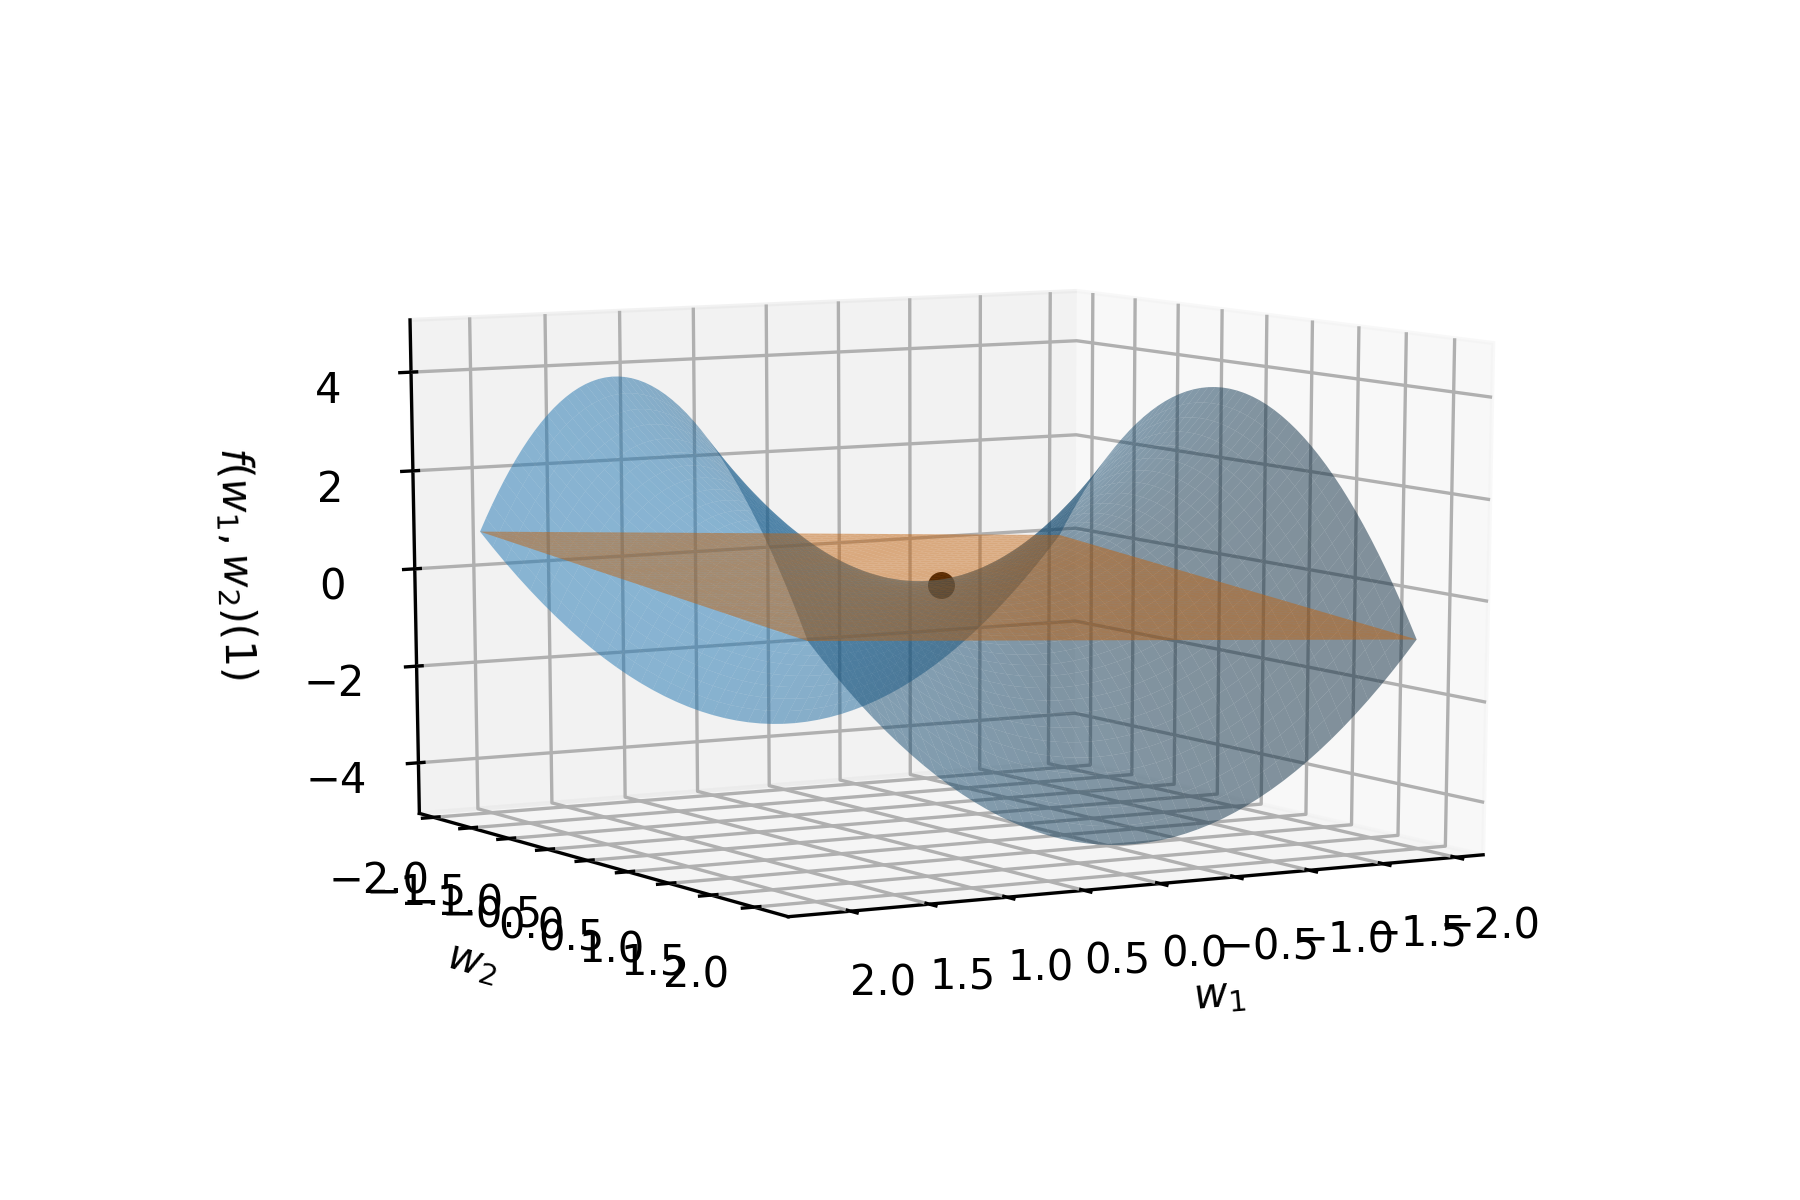
\includegraphics[width=.5\linewidth]{Imgs/Linearized_Model/visualize_linearized_0.1.png}}\hfill
    \subfloat[$\alpha = 10^1$]{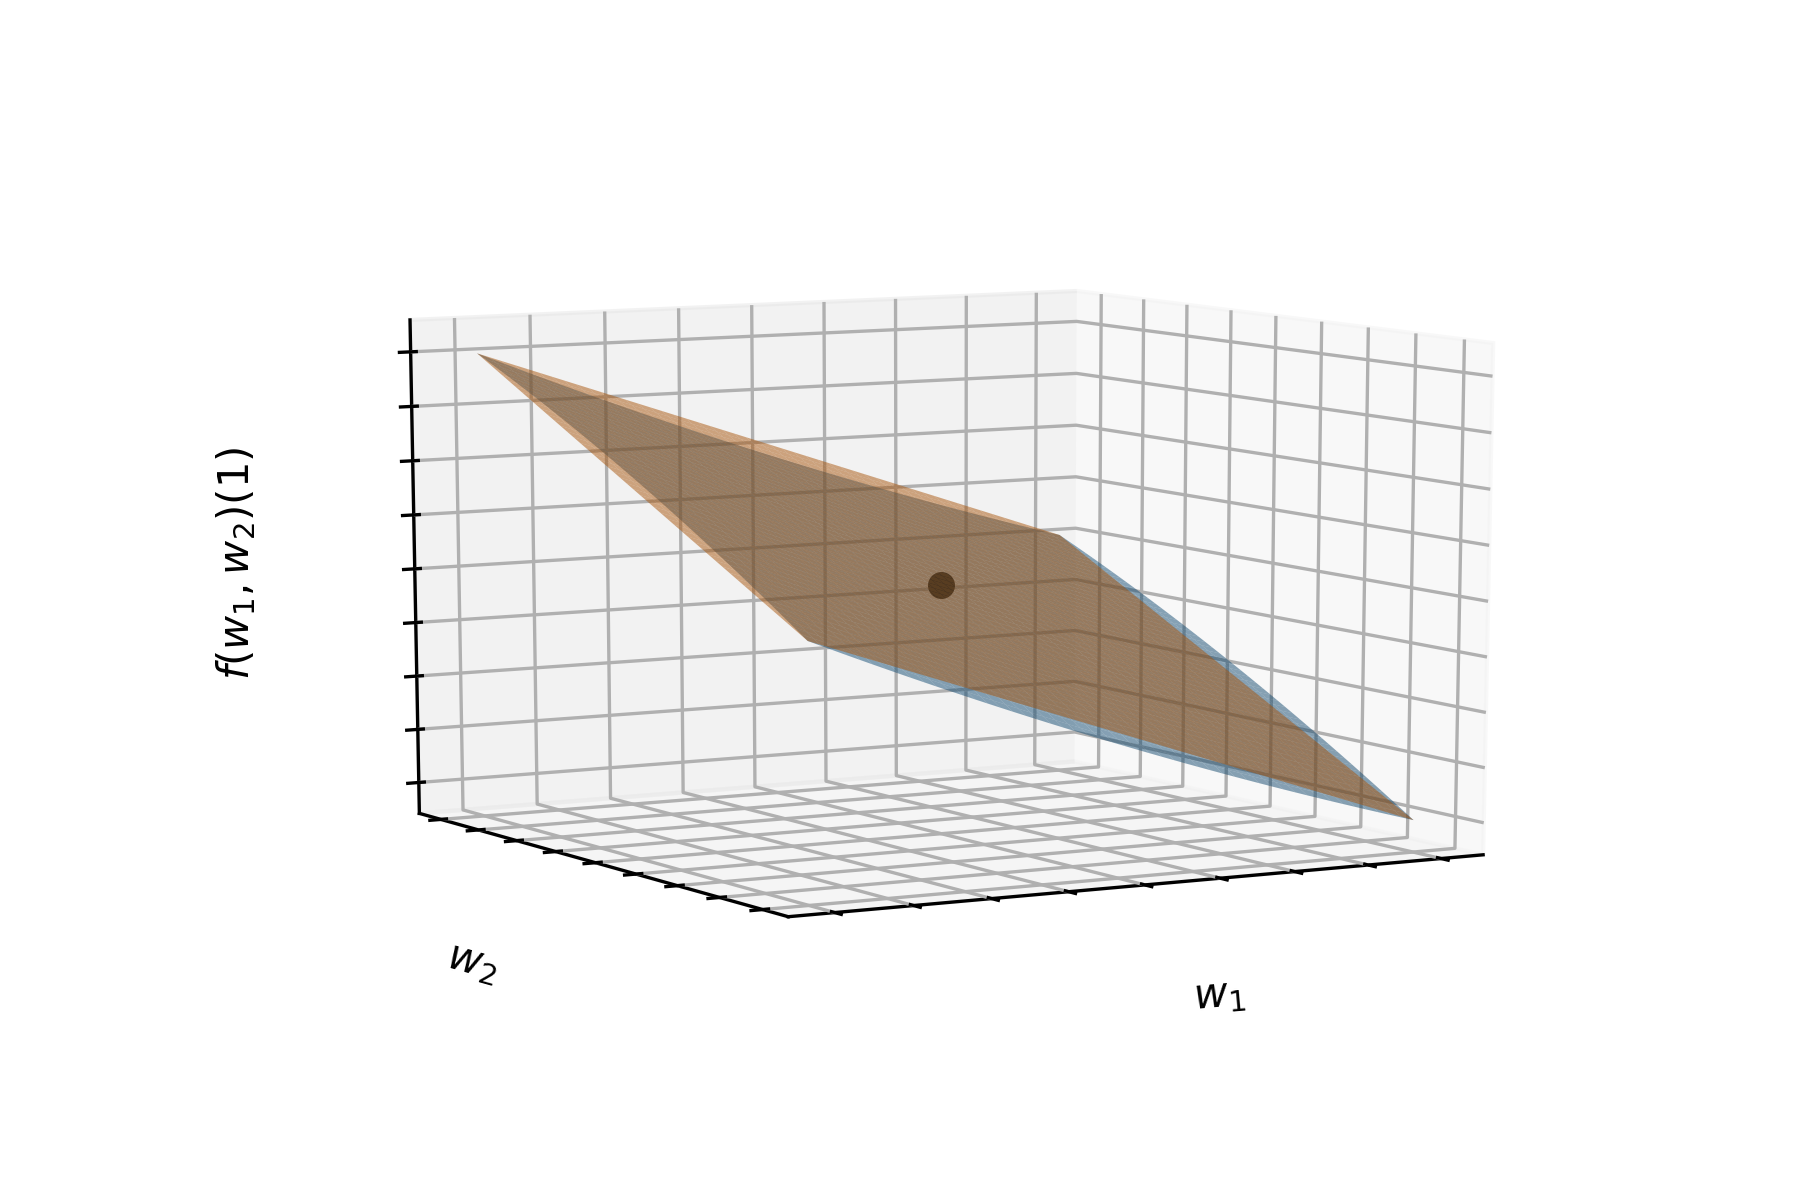
\includegraphics[width=.5\linewidth]{Imgs/Linearized_Model/visualize_linearized_10.png}}
    \caption{The linear regression model $f(\boldsymbol{w}, \boldsymbol{x})$ with one dimensional input $\boldsymbol{x} = 1$ and weights $\boldsymbol{w} = (w_1, w_2)$ initialized at $\boldsymbol{w}_{\alpha}(0) = \alpha \mathbbm{1}$. The original linear regression model $f(w_1, w_2)(1)$ is plotted in blue, and the linearized model $\bar{f}(w_1, w_2)(1)$ is in orange.}\label{img:linearization}
\end{figure}

Now that we have given exact characterizations of the kernel and rich limits for the linear regression problem, we wish to empirically demonstrate the transition between the two limits. Our first demonstration aims to represent the relationship between the original model $f(\boldsymbol{w}, \boldsymbol{x}) = \sum_{i=1}^n (\boldsymbol{w}_{i,+}^2 - \boldsymbol{w}_{i,-}^2)\boldsymbol{x}_i$ and the linearized model $\bar{f}(\boldsymbol{w}, \boldsymbol{x}) = \langle \varphi(\boldsymbol{x}), \boldsymbol{w} - \boldsymbol{w}_{\alpha}(0) \rangle = 2\alpha \langle \boldsymbol{x} , \boldsymbol{w}_+ -  \boldsymbol{w}_-\rangle$ with initialization $\boldsymbol{w}_{\alpha}(0) = \alpha \mathbbm{1}$. In particular, we know from Section \ref{defkernelrich} that as $\alpha \rightarrow \infty$, the gradient flow $(\boldsymbol{w}_{\alpha}(t))_{t \geq 0}$ is identical to $(\boldsymbol{\bar{w}}_{\alpha}(t))_{t \geq 0}$ with $\boldsymbol{w}_{\alpha}(0) = \boldsymbol{\bar{w}}_{\alpha}(0) = \alpha \mathbbm{1}$. And so we should observe that for fixed $\boldsymbol{x} \in \mathcal{X}$, $f(\boldsymbol{w}, \boldsymbol{x})$ is approximately equal to $\bar{f}(\boldsymbol{w}, \boldsymbol{x})$ as a function of $\boldsymbol{w} \in \mathbb{R}^p$ around the initialization $\boldsymbol{w}_{\alpha}(0) = \alpha \mathbbm{1}$. Conversely, as $\alpha \rightarrow 0$ we should observe that for fixed $\boldsymbol{x}$, $f(\boldsymbol{w}, \boldsymbol{x})$ is differs substantially from $\bar{f}(\boldsymbol{w}, \boldsymbol{x})$ around $\boldsymbol{w}_{\alpha}(0) = \alpha \mathbbm{1}$.

Since $\boldsymbol{w}$ increases quickly in dimension as $n$ grows, we consider the case of $n =1$. That is, we have a linear regression model with a single slope coefficient $\beta_{\boldsymbol{w}} = \boldsymbol{w}_{+, 1}^2 - \boldsymbol{w}_{-, 1}^2$. For simplicity, let us define $w_1 := \boldsymbol{w}_{+, 1}$, $w_2 := \boldsymbol{w}_{-, 1}$, and so we can view $f$ as a neural network with a one-dimensional input $x$ and two weights $w_1, w_2$. For our demonstrations, we choose the input $x = 1$ to be fixed. And so we are interested in the functions $f(w_1, w_2)(1), \bar{f}(w_1, w_2)(1): \mathbb{R}^2 \rightarrow \mathbb{R}$ mapping from the parameter space to the network output.

In Figure \ref{img:linearization}, we plot each of $f(w_1, w_2)(1)$ and $\bar{f}(w_1, w_2)(1)$ on the square grid $[\alpha - 2, \alpha + 2] \times [\alpha - 2, \alpha + 2]$ for $\alpha = 10^{-1}, 10^1$. Notice that the initialization $\boldsymbol{w}_{\alpha}(0) = \alpha \mathbbm{1}$ is at the center of this grid, and the black point represents $f(w_1, w_2)(1)$ evaluated at its initialization, $(\boldsymbol{w}_{\alpha}(0), f(\boldsymbol{w}_{\alpha}(0))(1)) = (\alpha \mathbbm{1}, 0)$. For all $\alpha \in \mathbb{R}_{++}$, $f$ is equal to $\bar{f}$ at its initialization: $f(\boldsymbol{w}_{\alpha}(0))(1) = \bar{f}(\boldsymbol{w}_{\alpha}(0))(1)$. And for $\alpha = 10^1$, we see that $|f(w_1, w_2)(1) - \bar{f}(w_1, w_2)(1) |$ is small for $\| (w_1, w_2) - \alpha \mathbbm{1} \|_2 > 0$, meaning $f$ is close to the affine model $\bar{f}$ around $\boldsymbol{w}_{\alpha}(0) = \alpha \mathbbm{1}$. On the other hand, for $\alpha = 10^{-1}$ we observe that $|f(w_1, w_2)(1) - \bar{f}(w_1, w_2)(1)|$ is large for $\| (w_1, w_2) - \alpha \mathbbm{1} \|_2 > 0$. That is, $f$ is highly nonlinear in $(w_1, w_2)$ about $\boldsymbol{w}_{\alpha}(0) = \alpha \mathbbm{1}$, and so is far from its linearization around $\boldsymbol{w}_{\alpha}(0)$, $\bar{f}$.

Letting the initialization scale $\alpha$ vary between $10^{-1}$ and $10^{1}$, we provide an even clearer representation of the relationship between the original model $f(w_1, w_2)(1)$ and the linearization of $f$ around $\boldsymbol{w}_{\alpha}(0) = \alpha \mathbbm{1}$, $\bar{f}(w_1, w_2)(1)$, in Figure \ref{gif:linearization}. Once again, we take the grid of input weights to be the region $[\alpha - 2, \alpha + 2] \times [\alpha - 2, \alpha + 2]$ containing $\boldsymbol{w}_{\alpha}(0)$.

\begin{figure}[H]
\animategraphics[loop, controls, width=\textwidth]{10}{Imgs/Linearized_Model/GIF_imgs/visualize_linearized_}{0}{99}
\caption{The linear regression model $f(w_1, w_2)(1)$ (blue) and the corresponding linearized model $\bar{f}(w_1, w_2)(1)$ (orange) for initialization scale $10^{-1} < \alpha < 10^1$.}\label{gif:linearization}
\end{figure}

From our illustrations, it is evident that for $\alpha \ll 1$, the gradient flow on $L(h(\boldsymbol{w}))$ with initialization $\boldsymbol{w}_{\alpha}(0) = \alpha \mathbbm{1}$ would result in quite a different model than that resulting from the gradient flow on $L(\bar{h}(\boldsymbol{w}))$ with $\boldsymbol{\bar{w}}_{\alpha}(0) = \boldsymbol{w}_{\alpha}(0)$. But as $\alpha$ grows away from $0$, then $h$ approaches $\bar{h}$ around $\boldsymbol{w}_{\alpha}(0)$ and the two solutions achieved by gradient flow $\lim_{t \to \infty} \boldsymbol{w}(t)$,  $\lim_{t \to \infty} \boldsymbol{\bar{w}}(t)$ are nearly identical.


\subsection{The Neural Tangent Kernel}\label{visualizeNTK}

The next aspect of the kernel and rich limits that we wish to illustrate is the neural tangent kernel (NTK). Recall that in Section \ref{linregmodel} we derived the NTK corresponding to the linear regression model at $\boldsymbol{w}_{\alpha}(0)$ to be
\begin{align*}
K(\boldsymbol{x}_1, \boldsymbol{x}_2) &= \left\langle \nabla_{\boldsymbol{w}}f(\boldsymbol{w}, \boldsymbol{x}_1)|_{\boldsymbol{w} = \boldsymbol{w}_{\alpha}(0)}, \nabla_{\boldsymbol{w}}f(\boldsymbol{w}, \boldsymbol{x}_2)|_{\boldsymbol{w} = \boldsymbol{w}_{\alpha}(0)} \right\rangle\\
&= \left\langle 2\alpha 
    \begin{bmatrix}
        \boldsymbol{x}_1\\
        -\boldsymbol{x}_1
    \end{bmatrix}, 2\alpha 
    \begin{bmatrix}
        \boldsymbol{x}_2\\
        -\boldsymbol{x}_2
    \end{bmatrix} \right\rangle\\
&= 8\alpha^2 \langle \boldsymbol{x}_1, \boldsymbol{x}_2 \rangle \quad \boldsymbol{x}_1, \boldsymbol{x}_2 \in \mathcal{X},
\end{align*}
which is just proportional to the $\ell^2$ kernel \cite{woodworth2020kernel}. One will also recall our discussion in Section \ref{kernelmethod} that since $h$ is unbiased at its initialization $\boldsymbol{w}_{\alpha}(0) = \alpha \mathbbm{1}$ and $L$ is the mean-squared error, then the gradient flow on $L(h(\boldsymbol{w}))$ is equivalent to a kernel method with kernel $K$ in the limit $\alpha \rightarrow \infty$. Put differently, in the kernel limit we are looking for a function $f^{\star}$ in the fixed feature space given by $\varphi(\boldsymbol{x})$ which is a global minimizer of $L(f), \ f \in (\mathbb{R}^n)^*$ \cite{wei2019regularization}.

\begin{figure}[H]
\centering
\subfloat[$\alpha = 10^{-1}$]{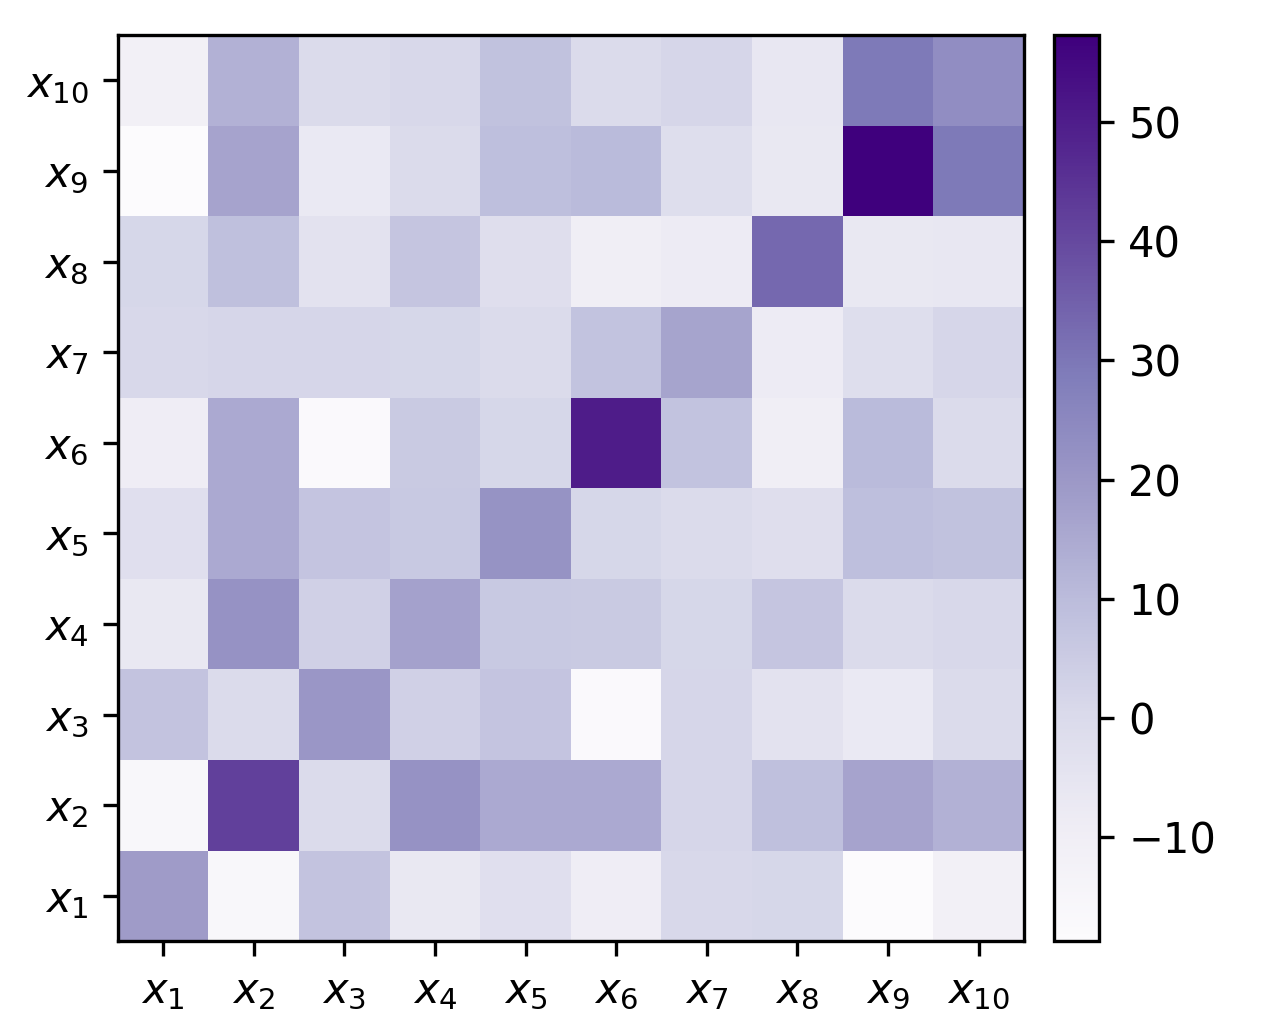
\includegraphics[width=.45\linewidth]{Imgs/NTK/NTK_0.1/NTK_0.1_change_total_cropped.png}}\hfill
\subfloat[$\alpha = 1$]{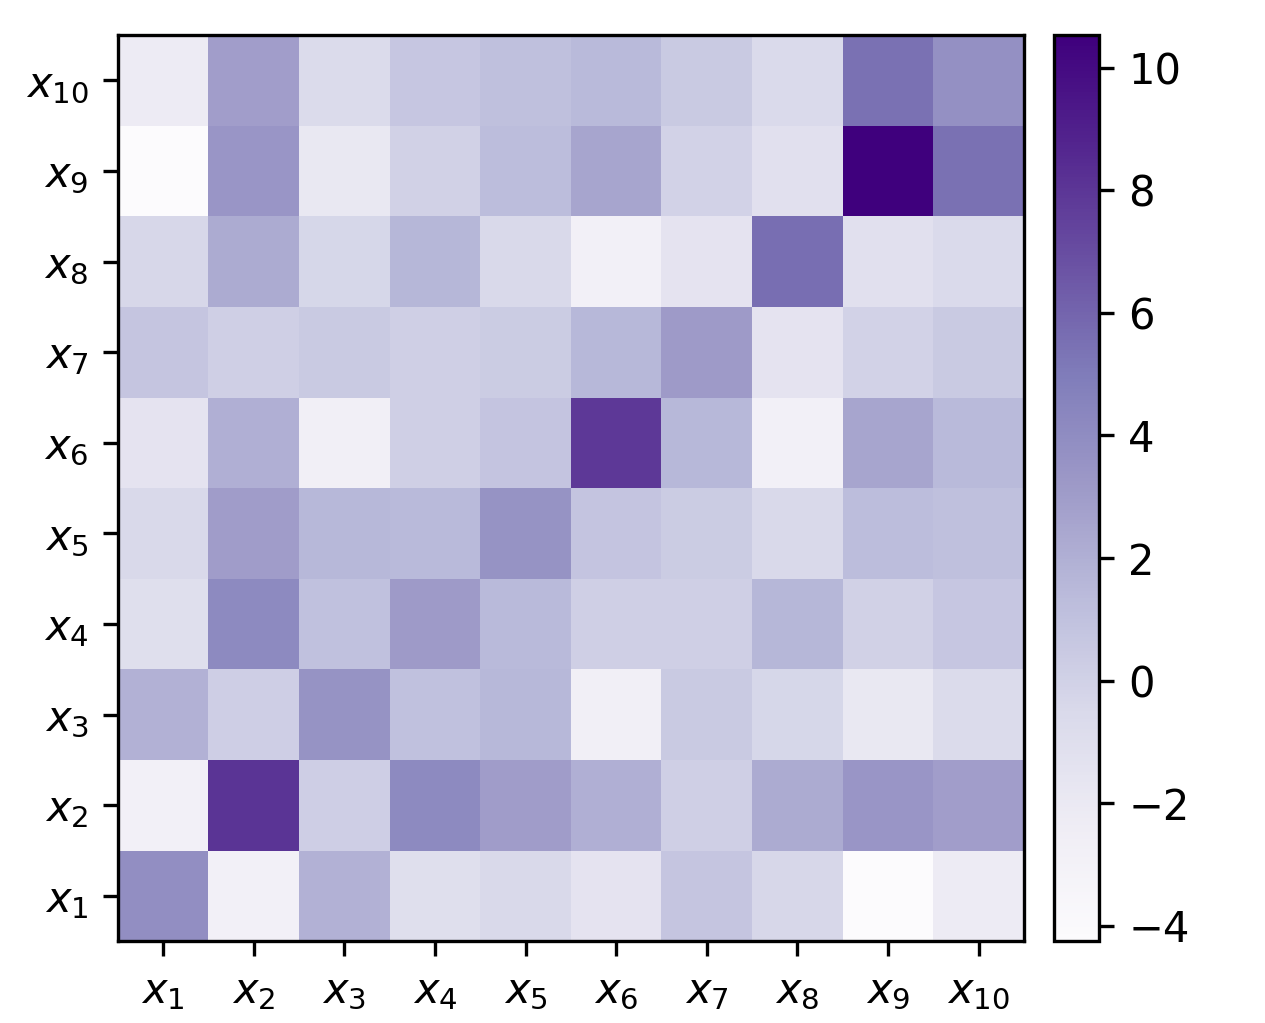
\includegraphics[width=.45\linewidth]{Imgs/NTK/NTK_1/NTK_1_change_total_cropped.png}}\par 
\subfloat[$\alpha = 10^{1}$]{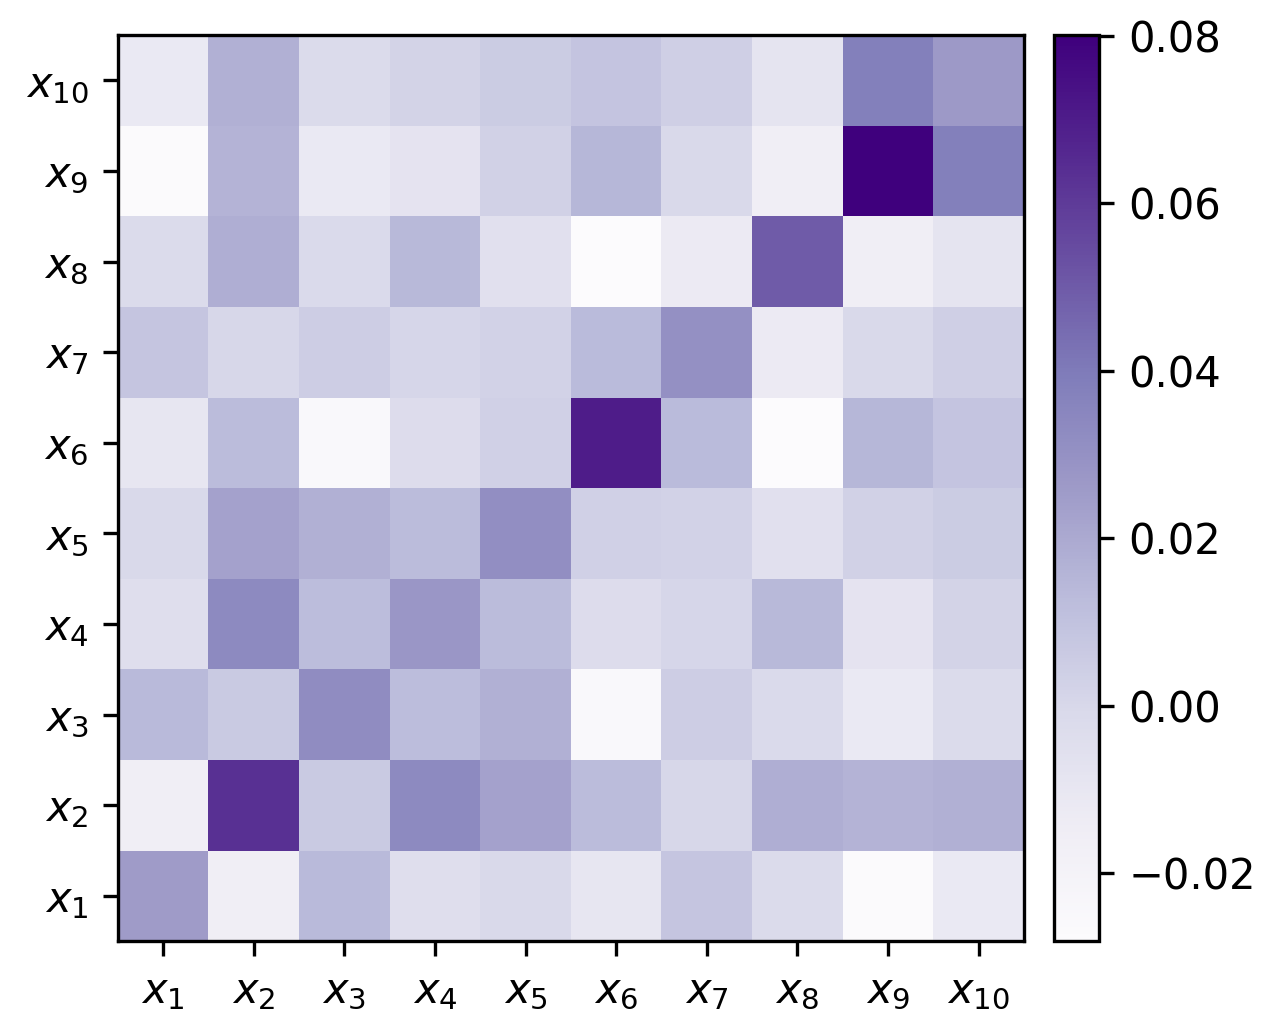
\includegraphics[width=.45\linewidth]{Imgs/NTK/NTK_10/NTK_10_change_total_cropped.png}}
\caption{The change in the neural tangent kernel (NTK) on the grid of $N= 10$ training points $\{ \boldsymbol{x}_i \}_{i=1}^{10}$ throughout training with gradient descent. For each of $\alpha = 10^{-1}, \ 1, \ 10^{1}$, we display the difference between the NTK at initialization $\boldsymbol{w}_{\alpha}(0)$ and at the end of training $\boldsymbol{w}_{\alpha}(t_{\text{end}})$.}\label{img:ntkchange}
\end{figure}

Summarizing our theoretical discussion, we know that in the kernel limit, the neural tangent kernel $K(\boldsymbol{x}_1, \boldsymbol{x}_2)$,\\ $\boldsymbol{x}_1, \boldsymbol{x}_2 \in \mathcal{X}$ should remain constant for all times $t \in \mathbb{R}_+$ in the gradient flow $(\boldsymbol{w}_{\alpha}(t))_{t \geq 0}, \ \boldsymbol{w}_{\alpha}(0) = \alpha \mathbbm{1}$ on $L(h(\boldsymbol{w}))$. Conversely, in the rich limit $\alpha \rightarrow 0$ we should observe that $K(\boldsymbol{x}_1, \boldsymbol{x}_2)$ evolves greatly throughout the gradient flow dynamics.

In order to demonstrate that the neural tangent kernel $K$ does, in fact, behave in this way, we consider gradient descent on $L(h(\boldsymbol{w}))$.  We once again start with $\boldsymbol{w}_{\alpha}(0) = \alpha \mathbbm{1}$ and let $(\boldsymbol{w}_{\alpha}(t))_{t \in \mathbb{N}\cup \{0\}}$ be our gradient descent path. As we previously hinted at in Section \ref{preliminaries}, gradient descent can be viewed as a forward Euler discretization of the gradient flow dynamics with positive stepsize $\eta > 0$. Accordingly, the gradient descent update is given by $\boldsymbol{w}_{\alpha}(t) = \boldsymbol{w}_{\alpha}(t-1) - \eta \nabla_{\boldsymbol{w}} L(h(\boldsymbol{w}))|_{\boldsymbol{w} = \boldsymbol{w}_{\alpha}(t-1)}$ for each $t \in \mathbb{N}$.

As for our training data, we consider $N=10$ points $\{ (\boldsymbol{x}_i, y_i) \}_{i=1}^N$ where each $\boldsymbol{x}_i \in \mathbb{R}^{n}$, $n = 20$ and $y_i \in \mathbb{R}$. This indeed satisfies the overparameterization assumption from Section \ref{linregmodel} since the dimension of the input space is much larger than the number of training points. As was done by Woodworth and colleagues in \cite{woodworth2020kernel}, we draw our input points according to $\boldsymbol{x}_i \overset{i.i.d.}{\sim} \mathcal{N}(\boldsymbol{0}, \mathbbm{I}_{n \times n})$. And to generate the corresponding set of response points, we compute $y_i = \langle \boldsymbol{x}_i, \boldsymbol{\beta} \rangle$, where $\boldsymbol{\beta}$ is generated according to the joint uniform distribution on $[-1, 1]^n$. Clearly, there is at least one vector, namely $\boldsymbol{\beta}_{\boldsymbol{w}} = \boldsymbol{\beta}$, such that $h = \langle \boldsymbol{\beta}, \boldsymbol{x} \rangle, \ \boldsymbol{x} \in \mathcal{X}$ is a global minimizer of the loss $L$.

Since our goal is to study the NTK in the kernel and rich regimes, we consider the gradient descent paths corresponding to initialization scales $\alpha = 10^{-1}, \ 1, \ 10^{1}$. To ensure that no one gradient descent path achieves smaller loss than the others, we stop training for each path once $L(h(\boldsymbol{w}_{\alpha}(t))) < 10^{-4}$. As one could likely predict, the challenge then becomes choosing a stepsize $\eta > 0$ such that $L(h(\boldsymbol{w}_{\alpha}(t)))$ converges within $10^{-4}$ of the global minimum. In particular, we would like to choose $\eta$ to be as small as possible while still achieving the desired convergence within a maximum of $10^4$ training epochs. A small $\eta$ is preferable because in the limit $\eta \rightarrow 0$, the gradient descent with stepsize $\eta$ reproduces the gradient flow dynamics. In the table below, we summarize our choice of stepsize $\eta$ for each gradient descent path:
\begin{table}[H]
\centering
\begin{tabular}{ c|c|c } 
$\alpha$ & $\eta$ & Number of Epochs to Convergence \\
\hline
$10^{-1}$ & $10^{-2}$ & $1001$ \\ 
$1$ & $10^{-3}$ & $757$ \\
$10^1$ & $10^{-4}$ & $77$
\end{tabular}
\caption{}\label{table:NTK}
\end{table}
Evidently, no single stepsize $\eta > 0$ works for all initialization scales. One aspect of our experiment that is potentially problematic is that the stepsize corresponding to the gradient descent path $\alpha = 10^{-1}$ is quite large. Therefore, it may be the case that the gradient descent path $(\boldsymbol{w}_{\alpha = 10^{-1}}(t))_{t \in \mathbb{N} \cup \{ 0 \}}$ is quite far from the corresponding gradient flow dynamics $(\boldsymbol{w}_{\alpha = 10^{-1}}(t))_{t\geq 0}$. With more computational power, it may be possible to achieve convergence with a smaller stepsize by increasing the maximum number of training epochs to be greater than $10^4$.

Before the first training epoch and after the final epoch we evaluate the neural tangent kernel $K_{\boldsymbol{w}_{\alpha}(t)}$ on the $10 \times 10$ grid of training points $\{ \boldsymbol{x}_i \}_{i=1}^N$. We do the same every ten training epochs in order to understand how the neural tangent kernel evolves throughout training. Note that $K_{\boldsymbol{w}_{\alpha}(t)}$ denotes the neural tangent kernel determined by the weight vector at epoch $t$ of training, $\boldsymbol{w}_{\alpha}(t)$. That is, 
\begin{align*}
    K_{\boldsymbol{w}_{\alpha}(t)}(\boldsymbol{x}_1, \boldsymbol{x}_2) &= \left\langle \nabla_{\boldsymbol{w}}f(\boldsymbol{w}, \boldsymbol{x}_1)|_{\boldsymbol{w} = \boldsymbol{w}_{\alpha}(t)}, \nabla_{\boldsymbol{w}}f(\boldsymbol{w}, \boldsymbol{x}_2)|_{\boldsymbol{w} = \boldsymbol{w}_{\alpha}(t)} \right\rangle, \quad \boldsymbol{x}_1, \boldsymbol{x}_2 \in \mathcal{X}.
\end{align*}

In Figure \ref{img:ntkchange}, we report the overall change in the NTK
\begin{align*}
   K_{\boldsymbol{w}_{\alpha}(t_{\text{end}})}(\boldsymbol{x}_i, \boldsymbol{x}_j) -  K_{\boldsymbol{w}_{\alpha}(0)}(\boldsymbol{x}_i, \boldsymbol{x}_j)
\end{align*}
on $\{ \boldsymbol{x}_i \}_{i=1}^N$ for the gradient descent paths with initialization scales $\alpha = 10^{-1}, \ 1, \ 10^1$. Here, $t_{\text{end}}$ denotes the final epoch of gradient descent as indicated in Table \ref{table:NTK}. Noticeably, for the large initialization scale $\alpha = 10$, the neural tangent kernel evaluated on the training grid changes very little from the beginning to the end of gradient descent. This empirically verifies our previous remarks about how we would expect the NTK to behave in the kernel regime, since in the kernel limit we have $K_{\boldsymbol{w}_{\alpha}(t)} = K_{\boldsymbol{w}_{\alpha}(0)}$ for all times $t \in \mathbb{R}_+$ in the gradient flow $(\boldsymbol{w}_{\alpha}(t))_{t \geq 0}, \ \boldsymbol{w}_{\alpha}(t) = \alpha \mathbbm{1}$ on $L(h(\boldsymbol{w}))$. Conversely, for the small initialization scale $\alpha = 10^{-1}$, we observe that the NTK varies greatly from the beginning to the end of training. That is, $K_{\boldsymbol{w}_{\alpha}(t_{\text{end}})}$ is very different from $K_{\boldsymbol{w}_{\alpha}(0)}$. Once again, this is how we would expect the NTK to evolve in the rich regime since the feature space determined by $\varphi_t(\boldsymbol{x}) = \nabla_{\boldsymbol{w}}f(\boldsymbol{w}, \boldsymbol{x})|_{\boldsymbol{w} = \boldsymbol{w}_{\alpha}(t)}$ is not fixed in time $t \in \mathbb{R}_+$ in the rich limit as it is in the kernel limit. From our experiment, we also see the interpolation between the kernel and rich regimes. At $\alpha = 1$, we remark that that the NTK exhibits behavior between the kernel and rich regimes. As we had previously commented, how the solutions reached by the gradient flow dynamics $(\boldsymbol{w}_{\alpha}(t))_{t \geq 0}$ $\boldsymbol{w}(0) = \alpha \mathbbm{1}$ vary between the rich $\alpha \rightarrow 0$ and kernel $\alpha \rightarrow \infty$ limits is considered rigorously by Woodworth and colleagues \cite{woodworth2020kernel}.

\begin{figure}[H]
\animategraphics[loop, controls, width=\textwidth]{10}{Imgs/NTK/NTK_0.1/GIF_imgs/linearized_NTK_0.1_}{0}{100}
\caption{The neural tangent kernel (NTK) evaluated on the grid of training points $\{ \boldsymbol{x}_i \}_{i=1}^N$ for every 10 epochs of gradient descent with initialization $\boldsymbol{w}_{\alpha = 10^{-1}}(0) = 10^{-1}\mathbbm{1}$.}\label{gif:ntk1}
\end{figure}

\begin{figure}[H]
\animategraphics[loop, controls, width=\textwidth]{10}{Imgs/NTK/NTK_1/GIF_imgs/linearized_NTK_1_}{0}{75}
\caption{The neural tangent kernel (NTK) evaluated on the grid of training points $\{ \boldsymbol{x}_i \}_{i=1}^N$ for every 10 epochs of gradient descent with initialization $\boldsymbol{w}_{\alpha = 1}(0) = \mathbbm{1}$.}\label{gif:ntk2}
\end{figure}

Although Figure \ref{img:ntkchange} certainly does portray how the neural tangent kernel changes from the beginning to the end of training, it does not fully capture how it evolves throughout training. To better understand the continuous time change of the NTK, we plot $K_{\boldsymbol{w}_{\alpha}(t)}$ on $\{ \boldsymbol{x}_i \}_{i=1}^N$ evaluated at every 10 epochs of gradient descent for the paths corresponding to $\alpha = 10^{-1}, \ 1$. We fix the scale of each plot Figure \ref{gif:ntk1} and Figure \ref{gif:ntk2} at $t = 0$ so that it does not automatically adjust at each evaluation of the NTK. Just as we would expect, the NTK corresponding to $\alpha = 10^{-1}$ experiences large relative changes, even at the end of training when $\boldsymbol{w}_{\alpha}(t)$ is close to a global minimum of the loss $L$. This is not the case for the gradient descent path corresponding to initialization scale $\alpha = 1$; in fact, it may appear as if the NTK does not change whatsoever. From Figure \ref{img:ntkchange} we know that this is not the case. Rather, for $\alpha = 1$ the changes in the NTK $K_{\boldsymbol{w}_{\alpha}(t)}$ are small relative to its scale at $\boldsymbol{w}_{\alpha}(0)$.

\subsection{The Model Weights}

\begin{figure}[H]
    \centering
    \subfloat[]{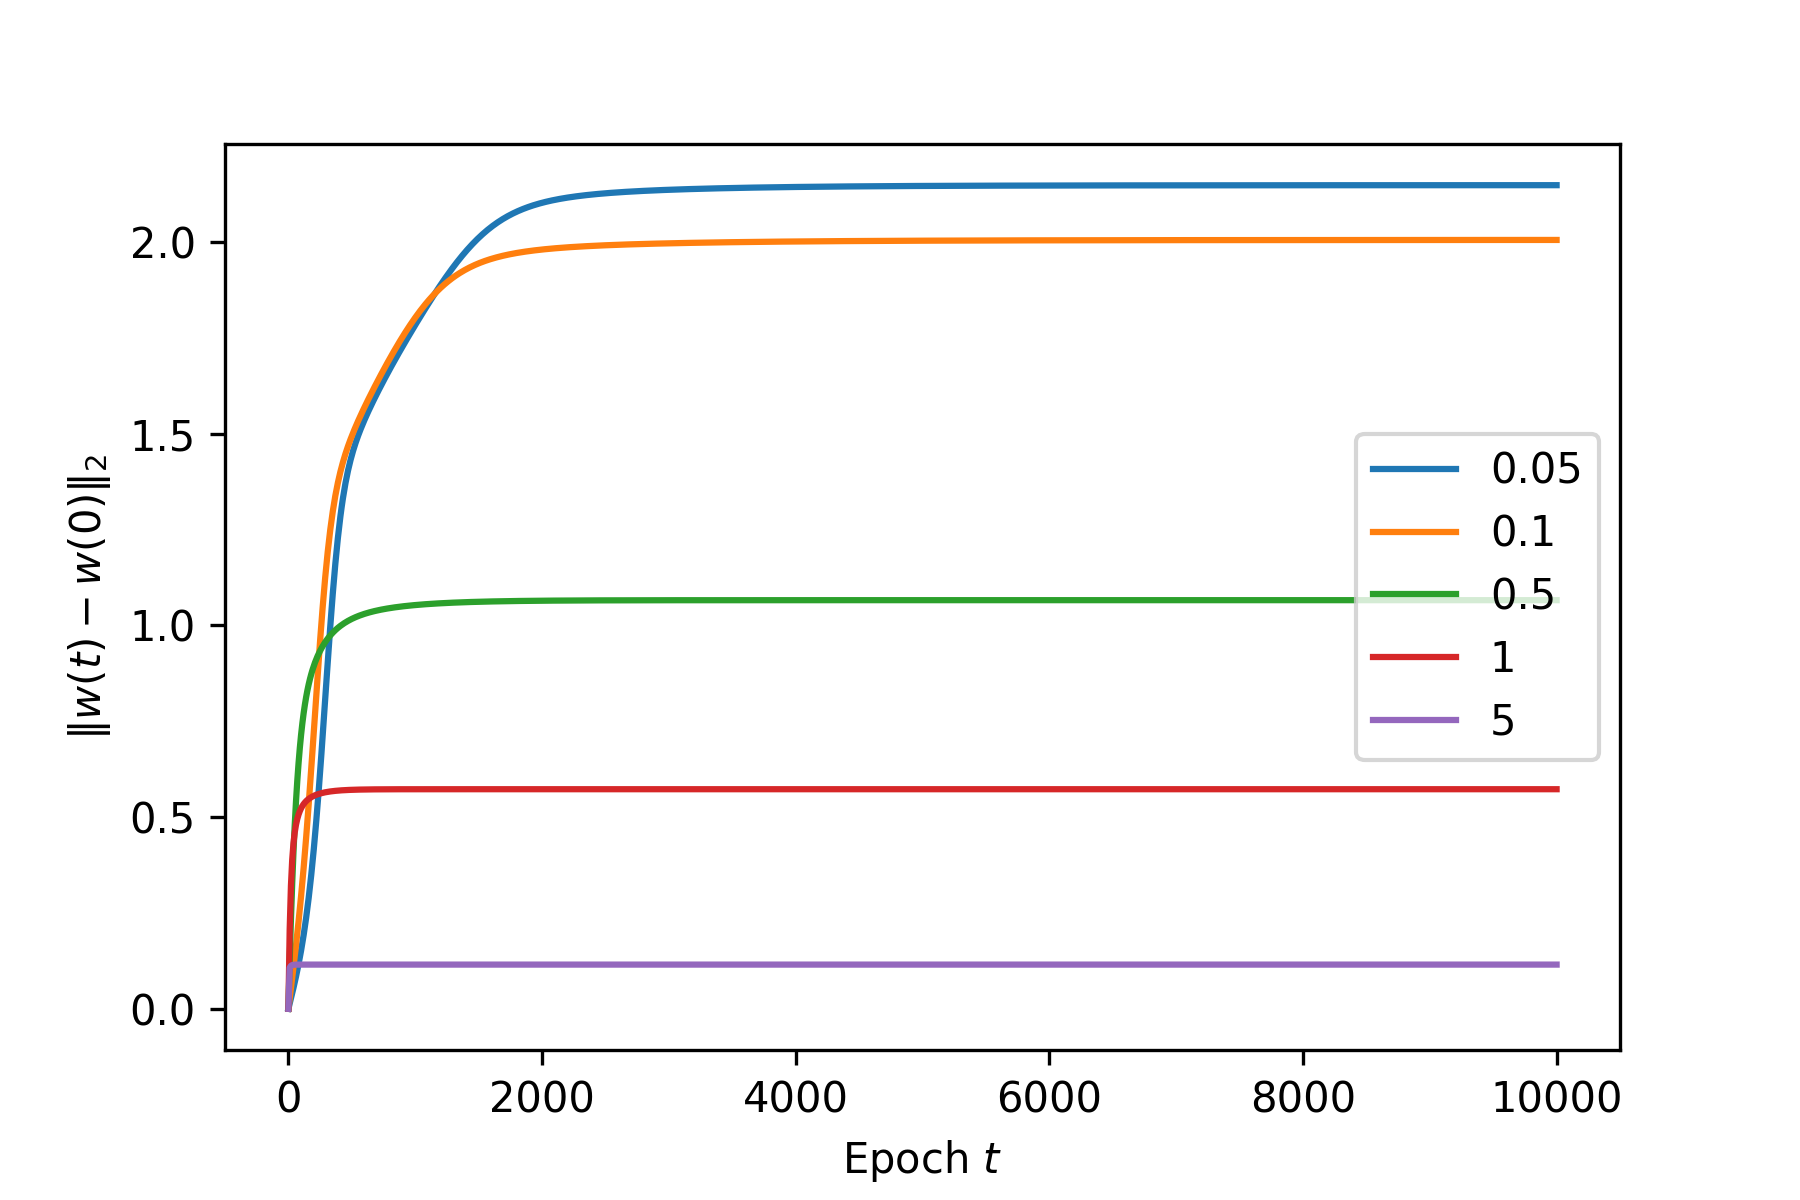
\includegraphics[width=.5\linewidth]{Imgs/Weights/visualize_change.png}\label{fig:weights:change}}\hfill
    \subfloat[]{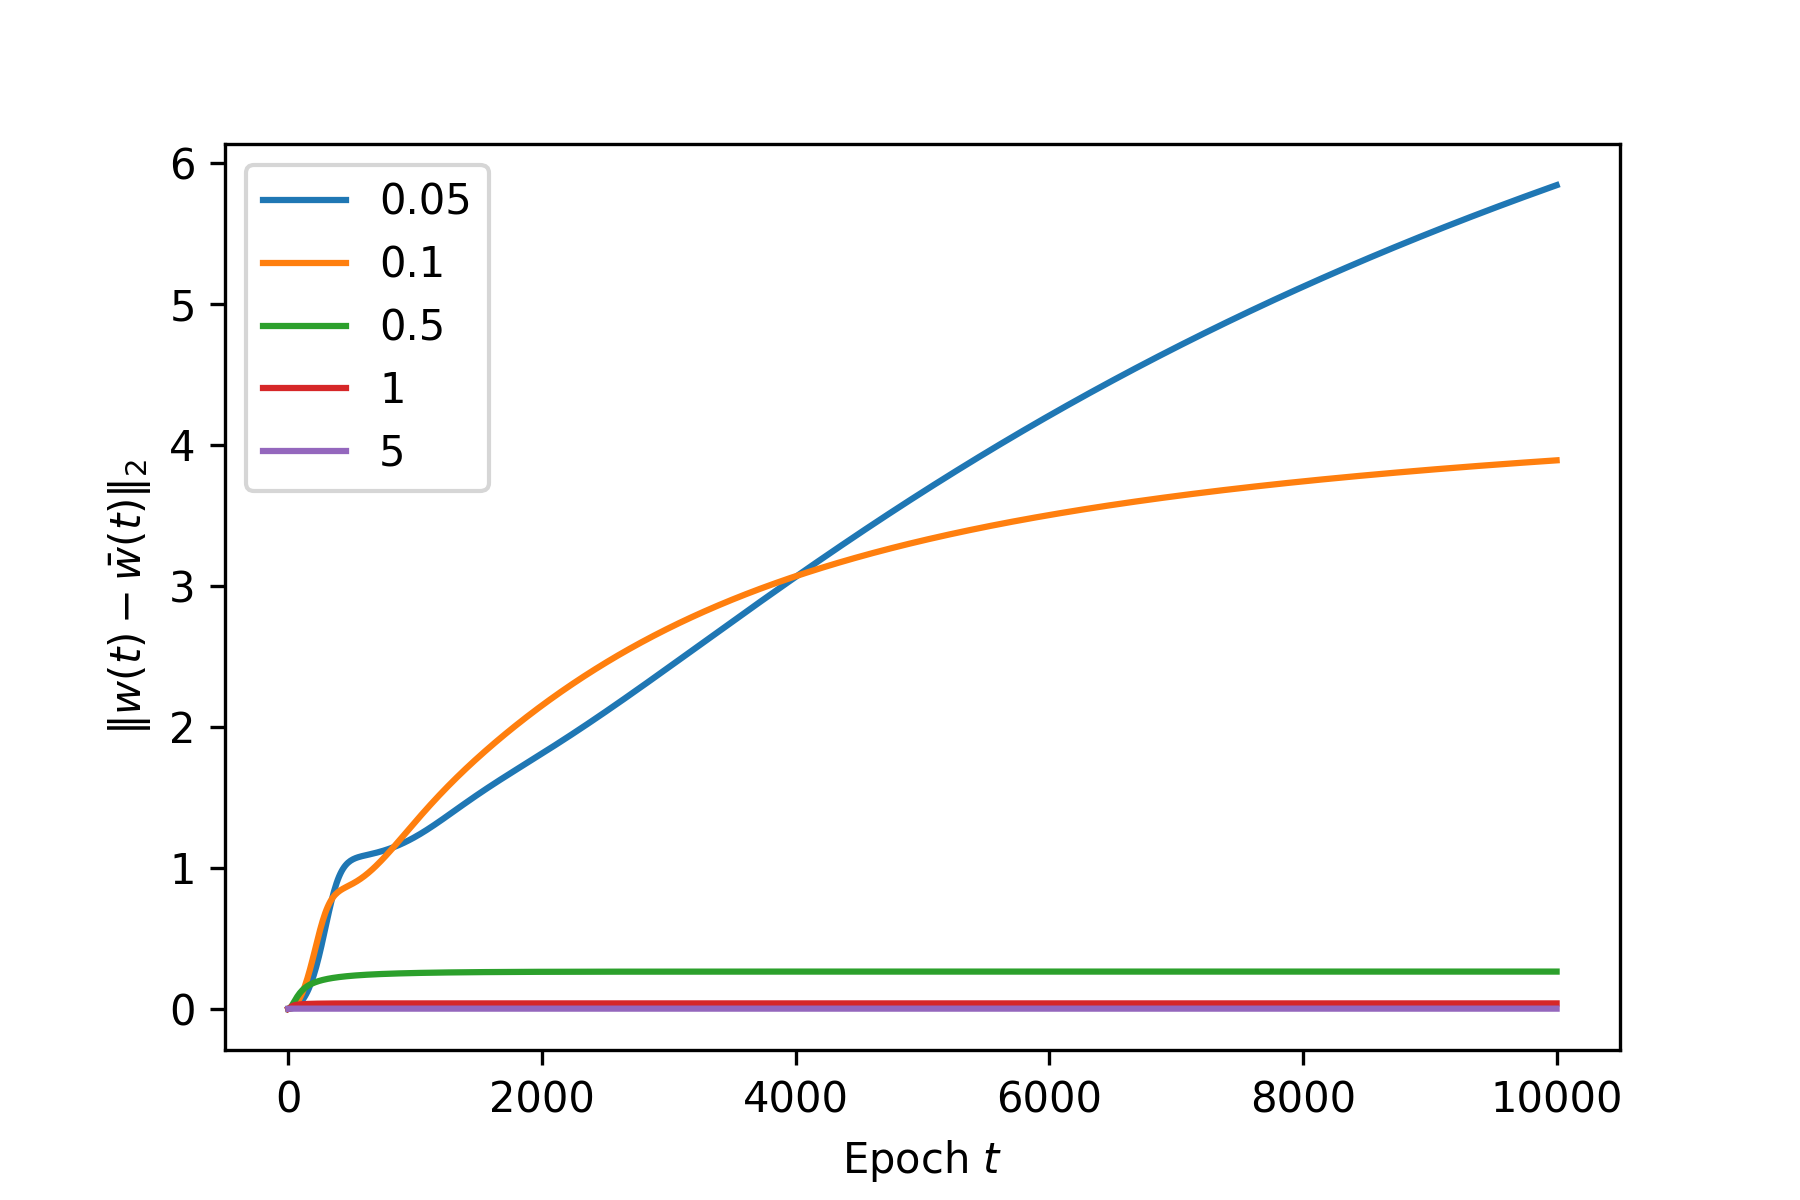
\includegraphics[width=.5\linewidth]{Imgs/Weights/visualize_weights.png}\label{fig:weights:diff}}
    \caption{(a) The $\ell^2$ distance between the weights of the model at epoch $t$ of gradient descent, $\boldsymbol{w}_{\alpha}(t)$, and at initialization $\boldsymbol{w}_{\alpha}(0) = \alpha \mathbbm{1}$. (b) The $\ell^2$ distance between the weights of the model $h$, $\boldsymbol{w}_{\alpha}(t)$, and those of the linearized model $\bar{h}$, $\boldsymbol{\bar{w}}_{\alpha}(t)$, at epoch $t$ of gradient descent. The initialization scale of each gradient descent path is indicated by the line color as reported in the plot legends.}\label{fig:weights}
\end{figure}

For our final demonstration of the kernel and rich limits in the linear regression problem, we consider how the weights of the model themselves $\boldsymbol{w}_{\alpha}(t)$ evolve throughout the gradient flow dynamics on $L(h(\boldsymbol{w}))$. From the theoretical results that we presented and discussed in Section \ref{kerneltheory}, we know that in the kernel limit $\alpha \rightarrow \infty$ it holds that $\| \boldsymbol{w}_{\alpha}(t) -  \boldsymbol{w}_{\alpha}(0) \|_2 \rightarrow 0$ as well as $\| \boldsymbol{w}_{\alpha}(t) -  \boldsymbol{\bar{w}}_{\alpha}(t) \|_2 \rightarrow 0$ for each $t \in \mathbb{R}_+$. The first result tells us that for all times $t \in \mathbb{R}_+$, the gradient flow path is asymptotically fixed at its initialization in the kernel limit. The second statement tells us that in the kernel limit, gradient flow on the original objective $L(h(\boldsymbol{w}))$ is equivalent to the gradient flow on $L(\bar{h}(\boldsymbol{w}))$. Using a similar setup to that in Section \ref{visualizeNTK}, we exhibit empirically that each of these two limits do, in fact, hold.


Just as in Section \ref{visualizeNTK}, we consider a training dataset of $N = 10$ points $\{(\boldsymbol{x}_i, y_i) \}_{i=1}^N$ with each $\boldsymbol{x}_i \in \mathbb{R}^n$, $n=20$ and $y_i \in \mathbb{R}$. The specifics of how we generate these $(\boldsymbol{x}_i, y_i)$ are exactly the same as in Section \ref{visualizeNTK}, and so we omit the details here. Similar to our experiment for the neural tangent kernel, we once again consider the gradient descent with initialization $\boldsymbol{w}_{\alpha}(0) = \alpha \mathbbm{1}$ , denoted $(\boldsymbol{w}_{\alpha}(t))_{t \in \mathbb{N}\cup\{0\}}$, as a discretization of the gradient flow dynamics. Here, we specifically look at the gradient descent paths corresponding to intialization scales $\alpha \in \{ 5\times10^{-2}, 10^{-1}, 5 \times 10^{-1}, 1, 5\}$. Unlike in the previous experiment, though, we fix a stepsize $\eta = 10^{-3}$ for each $\alpha$ and do not stop training early once $L(h(\boldsymbol{w}_{\alpha}(t))) < 10^{-4}$. Rather, we run each gradient descent path for a total of $10^4$ epochs. The reason for this is that we would like to compare $\boldsymbol{w}_{\alpha}(t)$ for these various $\alpha$, which we cannot do if the stepsize varies along with $\alpha$.

In order to demonstrate the first limit, $\| \boldsymbol{w}_{\alpha}(t) -  \boldsymbol{w}_{\alpha}(0) \|_2 \rightarrow 0$ as $\alpha \rightarrow \infty$, we store the network weights $\boldsymbol{w}_{\alpha}(t)$ both at the beginning of training $\boldsymbol{w}_{\alpha}(0) = \alpha \mathbbm{1}$ as well as after every 10 epochs of gradient descent. In Figure \ref{fig:weights:change}, we display the $\ell^2$ distance of $\boldsymbol{w}_{\alpha}(t)$ from the initialization $\boldsymbol{w}_{\alpha}(0)$ as a function of $t$. Just as we would expect under the aforementioned theory, the gradient descent path remains close to $\boldsymbol{w}(0)$ for all times $t$ whenever $\alpha$ is large. There ks In fact, for initialization scale $\alpha = 5$, we observe that $\boldsymbol{w}_{\alpha}(t)$ barely deviates from its initialization. On the opposite end of the paradigm, for $\alpha = 10^{-1}, \ 5 \times 10^{-2}$ we observe large changes in $\boldsymbol{w}_{\alpha}(t)$ throughout training. As we have previously explained, this active training is synonymous with the rich limit $\alpha \rightarrow 0$.

Furthermore, we are interested in the relationship between the gradient flow on $L(h(\boldsymbol{w}))$ and that on $L(\bar{h}(\boldsymbol{w}))$ in the kernel and rich limits. Since we have already computed $(\boldsymbol{w}_{\alpha}(t))_{t \in \mathbb{N} \cup \{0\}}$, then it remains to calculate $(\boldsymbol{\bar{w}}_{\alpha}(t))_{t \in \mathbb{N} \cup \{0\}}$, the gradient descent path on the linearized objective function $L(\bar{h}(\boldsymbol{w}))$ with initialization $\boldsymbol{\bar{w}}(0) = \alpha \mathbbm{1}$. Just as we did for the original objective, we run gradient descent for $10^4$ total training epochs with stepsize $\eta = 10^{-3}$. Likewise, we store the weights $\boldsymbol{\bar{w}}_{\alpha}(t)$ at the beginning of training and following every 10 gradient descent epochs. In Figure \ref{fig:weights:diff}, we report the $\ell^2$ distance between the gradient descent paths $\boldsymbol{w}_{\alpha}(t)$ and $\boldsymbol{\bar{w}}_{\alpha}(t)$ as a function of $t$. For large initialization scales $\alpha = 1, \ 5$, it is evident that $\boldsymbol{w}_{\alpha}(t)$ and $\boldsymbol{\bar{w}}_{\alpha}(t)$ are close for all times $t$. This supports the assertion that the gradient flow on $L(h(\boldsymbol{w}))$ is equivalent to that on the linearized objective $L(\bar{h}(\boldsymbol{w}))$ in the kernel limit $\alpha \rightarrow \infty$. On the contrary, for $\alpha = 5 \times 10^{-2}, 10^{-1}$ small, we see that $\| \boldsymbol{w}_{\alpha}(t) - \boldsymbol{\bar{w}}_{\alpha}(t) \|_2$ increases substantially throughout training. This suggests that gradient flow on the original objective $L(h(\boldsymbol{w}))$ is very different from that on the linearized objective $L(\bar{h}(\boldsymbol{w}))$ in the rich limit $\alpha \rightarrow 0$.

\section{Rich Training and Sparse Generalization}\label{richgeneralization}

Thus far, we have provided theoretical characterizations of the kernel and rich limits for neural network training and have demonstrated that these limits do, in fact, hold for the linear regression model considered in \cite{woodworth2020kernel}. What has been notably absent from our discussion, though, is why the distinction between kernel and rich training is meaningful. That is, why should one be conscious about whether they are training their network near the kernel limit or near the rich limit? 

To address this question, we must study the implicit biases of networks trained in the kernel and rich limits. One will recall that in Section \ref{linregmodel} we derived the explicit kernel and rich limits for the linear regression model from \cite{woodworth2020kernel}. In particular, the gradient flow solution in kernel limit is the minimum $\ell^2$ norm solution whereas the solution in the rich limit is the minimum $\ell^1$ norm solution. As Woodworth and colleagues point out, this result suggests benefits to training in the rich regime when one suspects that there is sparsity in the underlying model. This association of the rich limit with implicit $\ell^1$ regularization does not appear to be limited to the linear regression model, though. In Section \ref{richgeneralization}, we provide experimental results which suggest that for a particular sparse logistic regression problem, the rich limit similarly imposes $\ell^1$ regularization of the solution.

\subsection{The Sparse Linear Regression Problem}

For the first step in our examination of the implicit biases corresponding to the kernel and rich limits, we will look at the linear regression problem studied in Section \ref{linreg}. In particular, we know that for the model
\begin{align*}
    h(\boldsymbol{w}) = f(\boldsymbol{w}, \boldsymbol{x}) = \sum_{i=1}^n(\boldsymbol{w}_{+, i}^2 - \boldsymbol{w}_{-, i}^2)\boldsymbol{x}_i = \langle \boldsymbol{\beta}_{\boldsymbol{w}}, \boldsymbol{x} \rangle \qquad \boldsymbol{\beta}_{\boldsymbol{w}} = \boldsymbol{w}_+^2 -\boldsymbol{w}_-^2
\end{align*}
with loss function $L$ the mean-squared error, then gradient flow on the objective $L(h(\boldsymbol{w}))$, denoted\\ $(\boldsymbol{w}_{\alpha}(t))_{t \geq 0}$, with intialization $\boldsymbol{w}_{\alpha}(0) = \alpha \mathbbm{1}$ satisfies
\begin{align*}
    \lim_{t \to \infty} \boldsymbol{\beta}_{\boldsymbol{w}_{\alpha}(t)} = \argmin_{\boldsymbol{\beta} \in \mathbb{R}^n}  \| \boldsymbol{\beta} \|_2 \quad \text{as $\alpha \longrightarrow \infty$}, \qquad 
    \lim_{t \to \infty} \boldsymbol{\beta}_{\boldsymbol{w}_{\alpha}(t)} = \argmin_{\boldsymbol{\beta} \in \mathbb{R}_+^n}  \| \boldsymbol{\beta} \|_1 \quad \text{as $\alpha \longrightarrow 0$}.
\end{align*}

As we previously explained, this result suggests that training in the rich regime will outperform training in the kernel regime when there is sparsity in the underlying distribution $\rho$ from which the data $(\boldsymbol{x}_i, y_i)$ is drawn. When we say \enquote{outperform}, note that we are not referring to how well the model fits the training data. The gradient flow solutions reached in both the kernel and rich limits satisfy $\boldsymbol{X}\boldsymbol{\beta}^{\star} = \boldsymbol{y}$ for $\boldsymbol{\beta}^{\star} = \lim_{t \to \infty} \boldsymbol{\beta}_{\boldsymbol{w}_{\alpha}(t)}$, meaning they fit the training data exactly. Instead, we are referring to the generalization of the model on unseen data. If $(\boldsymbol{x}, y) \sim \rho$, then we can quantify how well a model $f(\boldsymbol{w}) \in \mathcal{F}$ generalizes as
\begin{align}\label{poprisk}
\mathbb{E}_{(\boldsymbol{x}, y) \sim \rho}[(y - f(\boldsymbol{w}, \boldsymbol{x}))^2],
\end{align}
which is the population risk corresponding to the square loss. That is, by computing the gradient flow solution of $L(h(\boldsymbol{w}))$ with $L$ the mean-squared error we are finding a minimizer of the empirical risk, which may or may not correspond to a small value of the population risk. It is also important to note that when we say that the distribution $\rho$ is \enquote{sparse}, we mean that $\boldsymbol{w} \mapsto \mathbb{E}_{(\boldsymbol{x}, y) \sim \rho}[(y - f(\boldsymbol{w}, \boldsymbol{x}))^2]$ is minimized by $\boldsymbol{w} \in \mathbb{R}^p$ sparse. Equivalently, we are stating that the true network parameters, those which minimize the population risk, are sparse. 

In order to demonstrate this desirable property of training near the rich limit for the linear regression model, we consider the following problem as it is formulated by Woodworth and colleagues. Suppose we have a training dataset of $N$ points $\{(\boldsymbol{x}_i, y_i)\}_{i=1}^N$, where each $\boldsymbol{x}_i \in \mathbb{R}^n$, $y_i \in \mathbb{R}$ for $n = 250$. We maintain our previous assumption that $N \leq n$ and more specifically that there exists many solutions to the system $\boldsymbol{X}\boldsymbol{\beta}_{\boldsymbol{w}} = \boldsymbol{y}$. The input data $\boldsymbol{x}_i$ is distributed according to $\mathcal{N}(\boldsymbol{0},\mathbbm{I}_{n \times n})$ and the corresponding output data is distributed according to $\mathcal{N}(\langle \boldsymbol{\beta}_{\boldsymbol{w}}, \boldsymbol{x}_i \rangle, \sigma^2)$ where $(\boldsymbol{\beta}_{\boldsymbol{w}})_i = 1/\sqrt{5}$ for $1 \leq i \leq 5$, $(\boldsymbol{\beta}_{\boldsymbol{w}})_i = 0$ otherwise. Here, $\sigma^2 = 10^{-2}$ is a constant which determines the amount of noise in the output data.

First, one should observe that the data we are considering is very high-dimensional. Consequently, with no prior knowledge of the true data distribution $\rho$, one would expect that they would need many training samples to achieve good generalization of $h(\lim_{t \to \infty} \boldsymbol{w}_{\alpha}(t))$. In spite of the high dimensionality of the input space, though, the underlying data distribution $\rho$ is specified such that $y_i$ is determined by merely the first five coordinates of $\boldsymbol{x}_i$. Put more rigorously, by choosing  $\boldsymbol{w} \in \mathbb{R}^{500}$ such that $(\boldsymbol{w}_+^2 - \boldsymbol{w}_-^2)_{1:5} = 1/\sqrt{5}$ and $\boldsymbol{w}_i = 0$ otherwise, then the corresponding network function $f(\boldsymbol{w})$ minimizes the population risk (\ref{poprisk}). And so we can theoretically minimize the population risk using a network with only 10 nonzero weights out of $2n = 500$ total and with weight vector satisfying $\| \boldsymbol{w} \|_1 = \sqrt{5}$.

Now that we have detailed the sparse regression problem from \cite{woodworth2020kernel}, we proceed to address how we will simulate the gradient flow on $L(h(\boldsymbol{w}))$. Just as in Section \ref{summarizekernel}, we approximate the gradient flow dynamics on $L(h(\boldsymbol{w}))$, $(\boldsymbol{w}_{\alpha}(t))_{t \geq 0}$, using the corresponding gradient descent path, $(\boldsymbol{w}_{\alpha}(t))_{t \in \mathbb{N} \cup \{ 0\}}$, with small stepsize $\eta = 3 \times 10^{-4}$. To ensure that we are fairly comparing the solution vectors $\boldsymbol{w}_{\alpha}(t_{\text{end}})$, we stop training once $L(h(\boldsymbol{w}_{\alpha}(t))) < 10^{-4}$. Since it might be the case, as we encountered in Section \ref{visualizeNTK}, that gradient descent converges very slowly to a global minimum of the objective function, we stop training after a maximum of $10^4$ epochs. 

\begin{figure}[H]
    \centering
    \subfloat[]{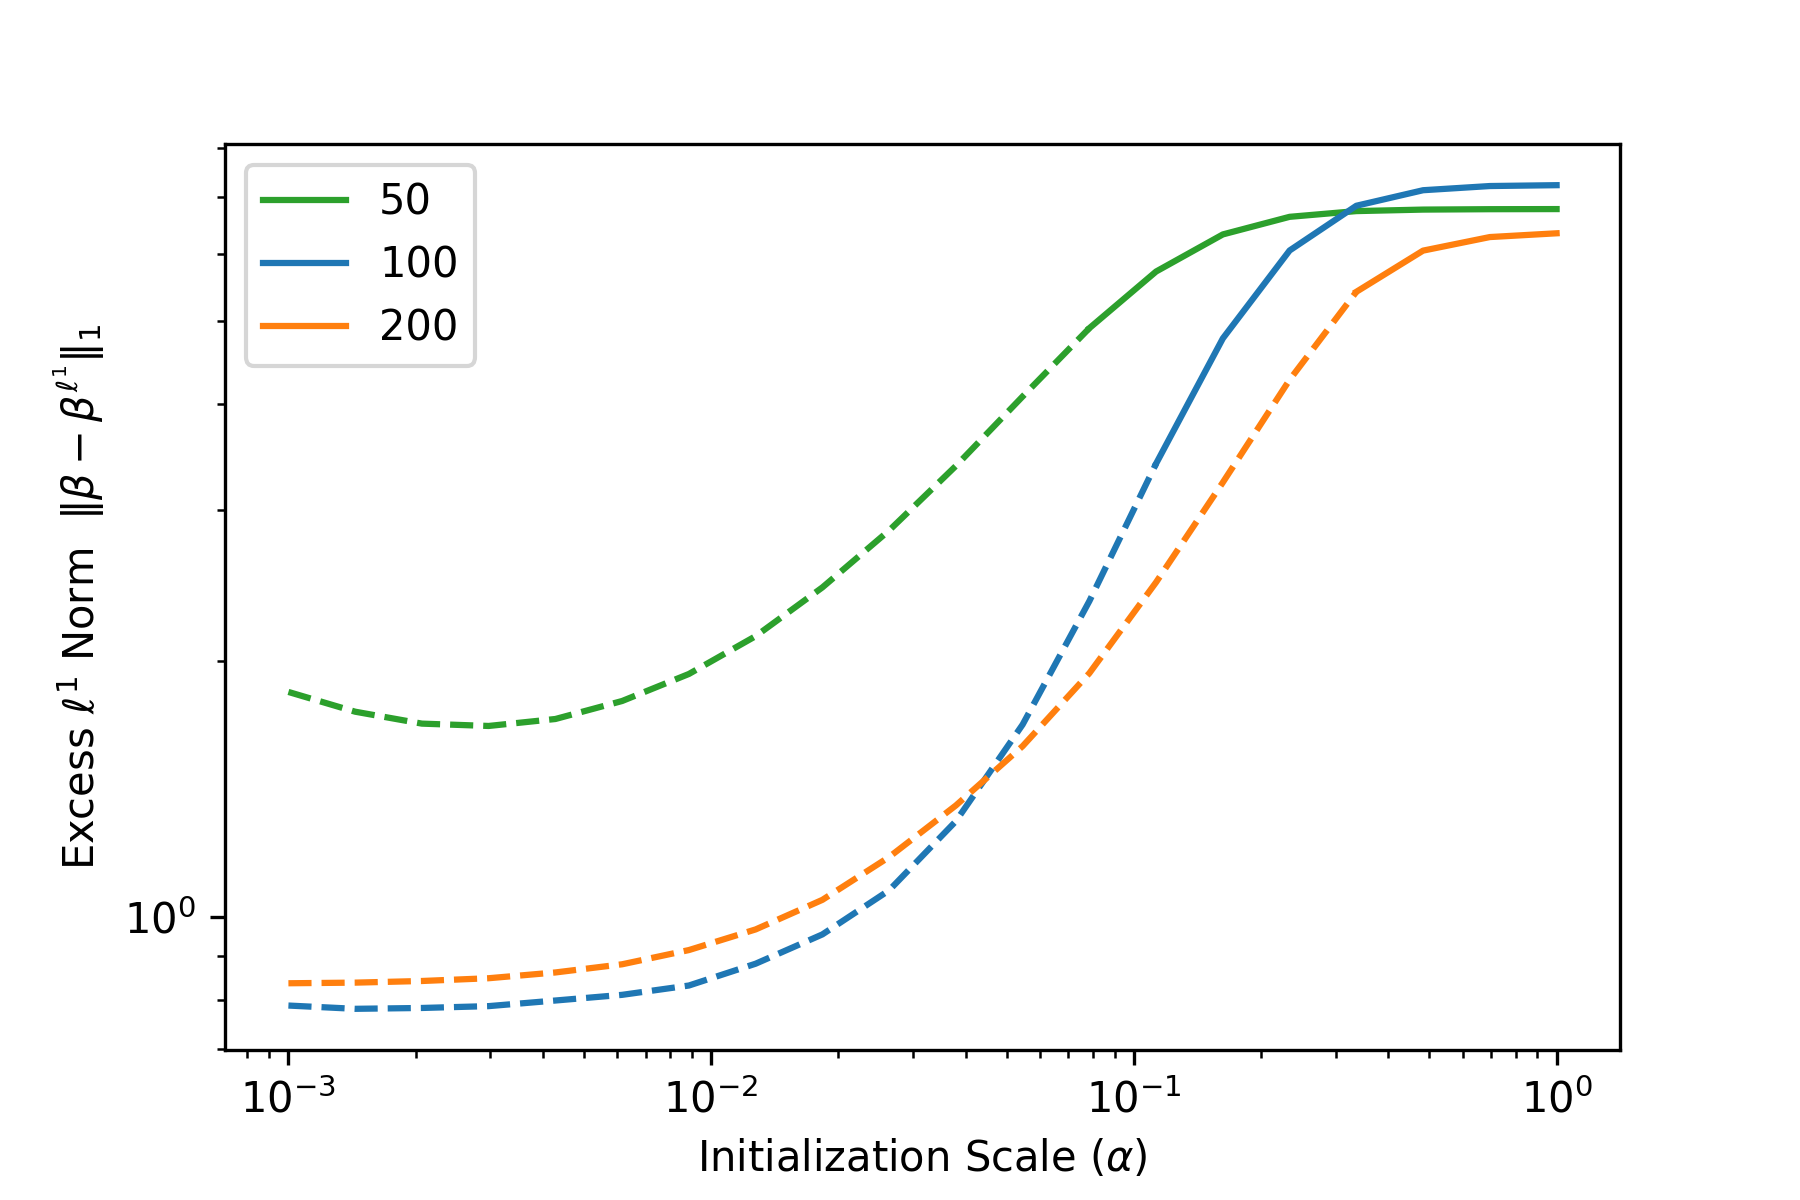
\includegraphics[width=.5\linewidth]{Imgs/Sparse Linear Regression/excess_l1_log_all.png}\label{fig:excessl1error}}\hfill
    \subfloat[]{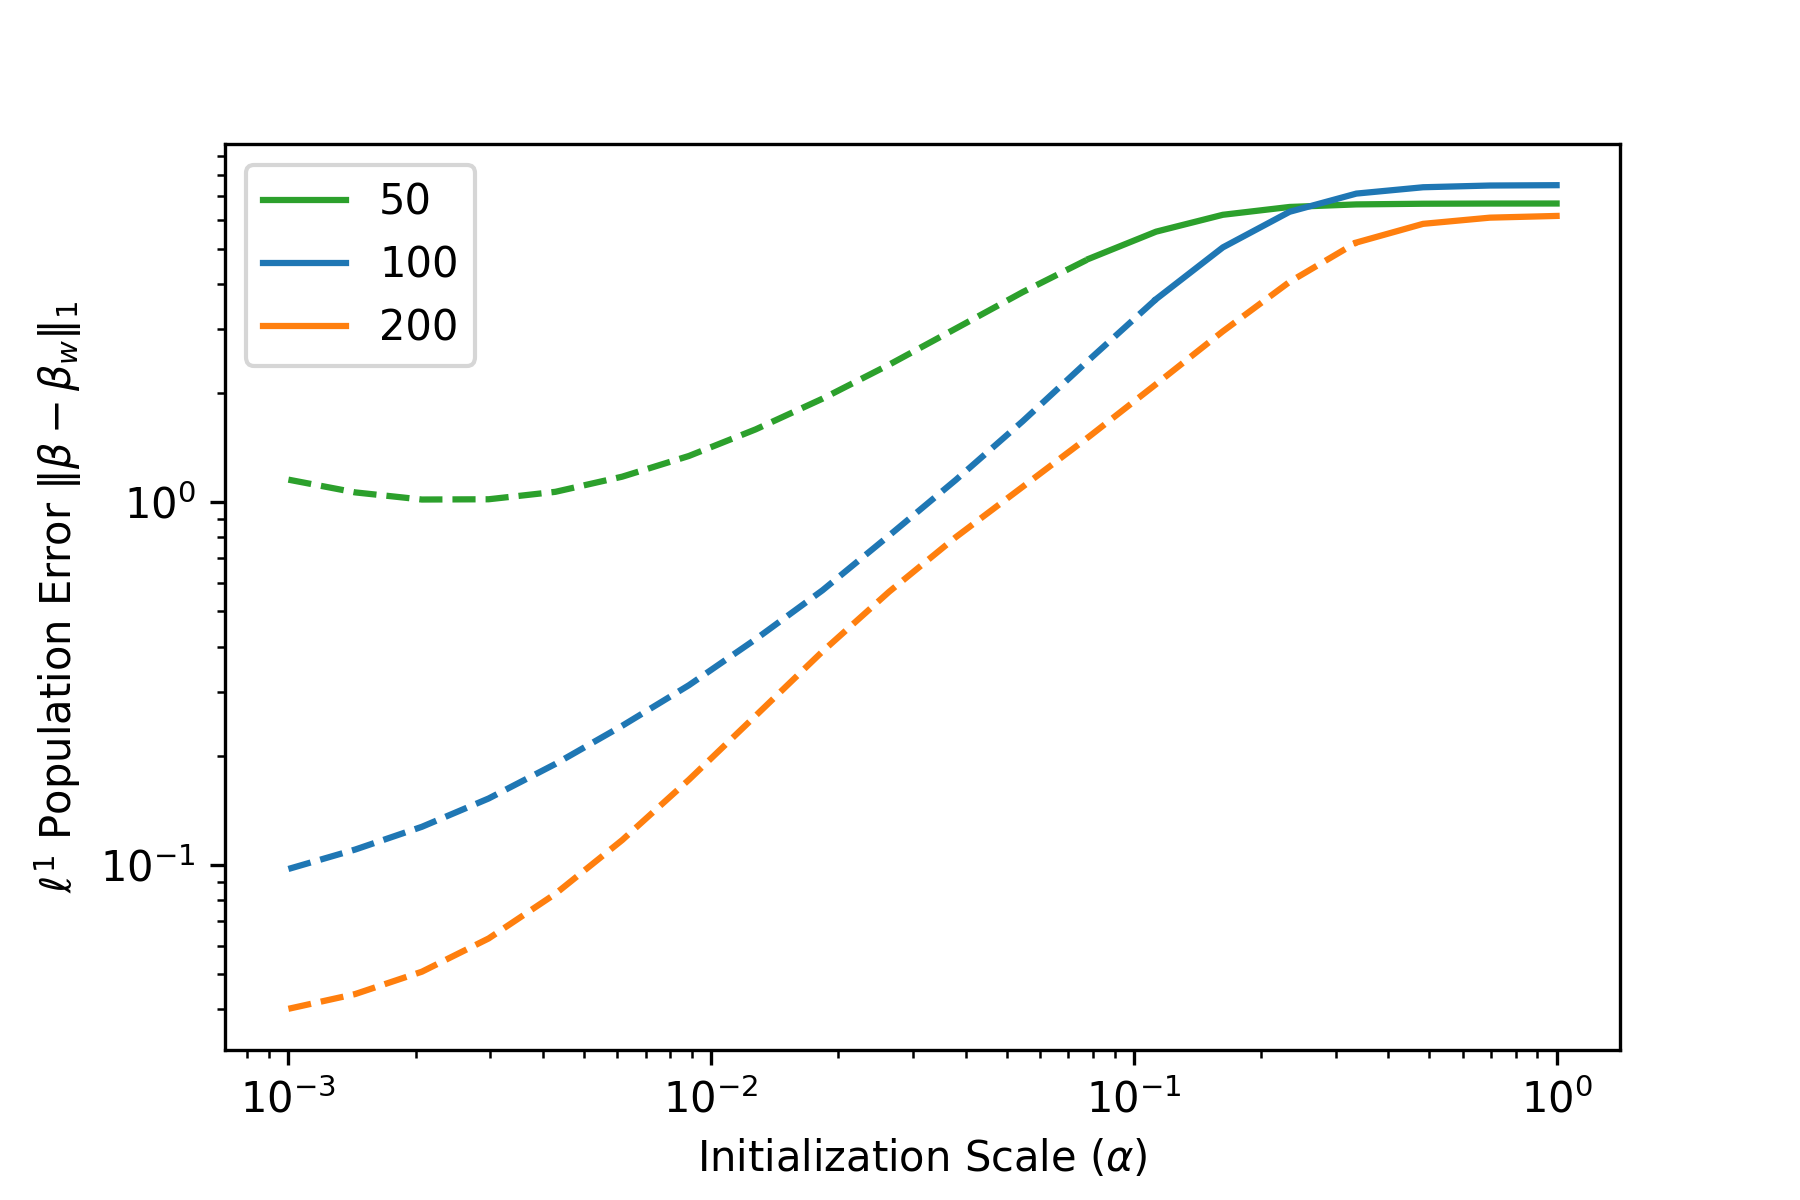
\includegraphics[width=.5\linewidth]{Imgs/Sparse Linear Regression/11_population_error_log_all.png}\label{fig:l1populationerror}}
    \caption{(a) The $\ell^1$ difference between the gradient descent solution $\boldsymbol{\beta}_{\boldsymbol{w}_{\alpha}(t_{\text{end}})}$ and the minimum $\ell^1$ solution $\argmin_{\boldsymbol{\beta} \in \mathbb{R}^n} \| \boldsymbol{\beta} \|_1, \ \boldsymbol{X} \boldsymbol{\beta}  = \boldsymbol{y}$, where $\boldsymbol{X} \in \mathbb{R}^{N \times n}$ is the matrix of training inputs $\{ \boldsymbol{x}_i \}_{i=1}^N$, $\boldsymbol{y} \in \mathbb{R}^N$ the vector of training outputs $\{y_i\}_{i=1}^N$. (b) The $\ell^1$ difference between the gradient descent solution and the ground truth vector $\boldsymbol{\beta}_{\boldsymbol{w}}$ from which the output data is generated. For each of (a) and (b), a dashed line indicates that the gradient descent path did not achieve the specified convergence.}\label{fig:l1error}
\end{figure}

Unlike in our previous experiments, though, we consider the gradient descent path both as a function of the number of training samples, $N$, as well as the initialization scale, $\alpha$. To be more specific, we evaluate the gradient descent path using a training dataset of $N = 50, \ 100,$ and $200$ points $\{ (\boldsymbol{x}_i, y_i) \}_{i=1}^N$. And for each fixed $N$, we choose $20$ logarithmically-spaced points on the interval $[10^{-3}, 1]$ for the initialization scale $\alpha$. Altogether, each combination of $N$ and $\alpha$ specifies a gradient descent path which we simulate as previously described.

In Figure \ref{fig:excessl1error}, we report the excess $\ell^1$ norm of the solution vector $\boldsymbol{\beta}_{\boldsymbol{w}_{\alpha}(t_{\text{end}})}$ reached by the gradient descent path $(\boldsymbol{w}_{\alpha}(t))_{t \in \mathbb{N}\cup \{0\}}$, $\boldsymbol{w}_{\alpha}(0) = \alpha \mathbbm{1}$. That is, we determine the minimum $\ell^1$ solution to the system $\boldsymbol{X} \boldsymbol{\beta} = \boldsymbol{y}$, denoted $\boldsymbol{\beta}^{\ell^1}$, and then calculate the $\ell^1$ difference between this vector and the gradient flow solution $\boldsymbol{\beta}_{\boldsymbol{w}_{\alpha}(t_{\text{end}})}$. From our plot, we see that for each of $N= 100, \ 200$, there is a clear pattern in which the gradient flow solution is far from the minimum $\ell^1$ solution for $\alpha =1$ (excess $\ell^1$ norm $\sim5$) but gets significantly closer to this solution as $\alpha$ shrinks towards zero (excess $\ell^1$ norm $\sim 8\times 10^{-1}$ for $\alpha = 10^{-3}$). From our theoretical results regarding the gradient flow solution for the linear regression model in the rich limit $\alpha \rightarrow 0$, this is what we would expect. More explicitly, we know that in the limit $\alpha \rightarrow 0$, the gradient flow solution on the objective $L(h(\boldsymbol{w}))$ with initialization $\boldsymbol{w}_{\alpha}(0) = \alpha \mathbbm{1}$ should correspond exactly to the minimum $\ell^1$ solution of the system $\boldsymbol{X} \boldsymbol{\beta} = \boldsymbol{y}$. On the other hand, since the gradient flow solution in the kernel limit $\alpha \rightarrow \infty$ corrresponds to the minimum $\ell^2$ solution, then $\boldsymbol{\beta}_{\boldsymbol{w}_{\alpha}(t_{\text{end}})}$ should not be close to $\boldsymbol{\beta}^{\ell^1}$ for $\alpha$ large.

While the excess $\ell^1$ norm suggests how far the gradient flow solution is from the minimum $\ell^1$ norm solution, we would also like to consider how far it is from the vector $\boldsymbol{\beta}_{\boldsymbol{w}}$ which minimizes the population risk. In Figure \ref{fig:l1populationerror} we present the $\ell^1$ population error, which is measured as the $\ell^1$ distance between $\boldsymbol{\beta}_{\boldsymbol{w}_{\alpha}(t_{\text{end}})}$ and $\boldsymbol{\beta}_{\boldsymbol{w}}$, where $\boldsymbol{\beta}_{\boldsymbol{w}}$ is the vector defined above which determines the distribution of $y_i$ (i.e. $(\boldsymbol{\beta}_{\boldsymbol{w}})_i = 1/\sqrt{5}$ for $1 \leq i \leq 5$, $(\boldsymbol{\beta}_{\boldsymbol{w}})_i = 0$ otherwise). One will notice that unlike $\boldsymbol{\beta}^{\ell^1}$, $\boldsymbol{\beta}_{\boldsymbol{w}}$ is not a solution to the system $\boldsymbol{X} \boldsymbol{\beta} = \boldsymbol{y}$ almost surely. This is a result of the small perturbations made to the output points $y_i$ from their mean $\langle \boldsymbol{\beta}_{\boldsymbol{w}}, \boldsymbol{x}_i \rangle$. Nonetheless, since $\boldsymbol{\beta}_{\boldsymbol{w}}$ is a minimizer of the population risk (\ref{poprisk}), then it is desirable that $\boldsymbol{\beta}_{\boldsymbol{w}_{\alpha}(t_{\text{end}})} \approx \boldsymbol{\beta}_{\boldsymbol{w}}$. Indeed, we observe that for $N = 100, \ 200$, the $\ell^1$ population error is small for $\alpha$ small: when $\alpha = 10^{-3}$, the $\ell^1$ population error is $\sim 10^{-1}$ with $N=100$ training samples and $\sim 4 \times 10^{-2}$ with $N=200$ training samples. Intuitively, we would suspect that  $\boldsymbol{\beta}_{\boldsymbol{w}_{\alpha}(t_{\text{end}})}$ should be close to $\boldsymbol{\beta}_{\boldsymbol{w}}$ for $\alpha$ small since $\boldsymbol{\beta}_{\boldsymbol{w}}$ itself is sparse. This finding informs how one should choose their initialization scale $\alpha$ to minimize the population risk when they believe that the underlying data distribution $\rho$ is sparse.

\begin{figure}[H]
    \centering
    \subfloat[$\alpha = 10^{-3}$]{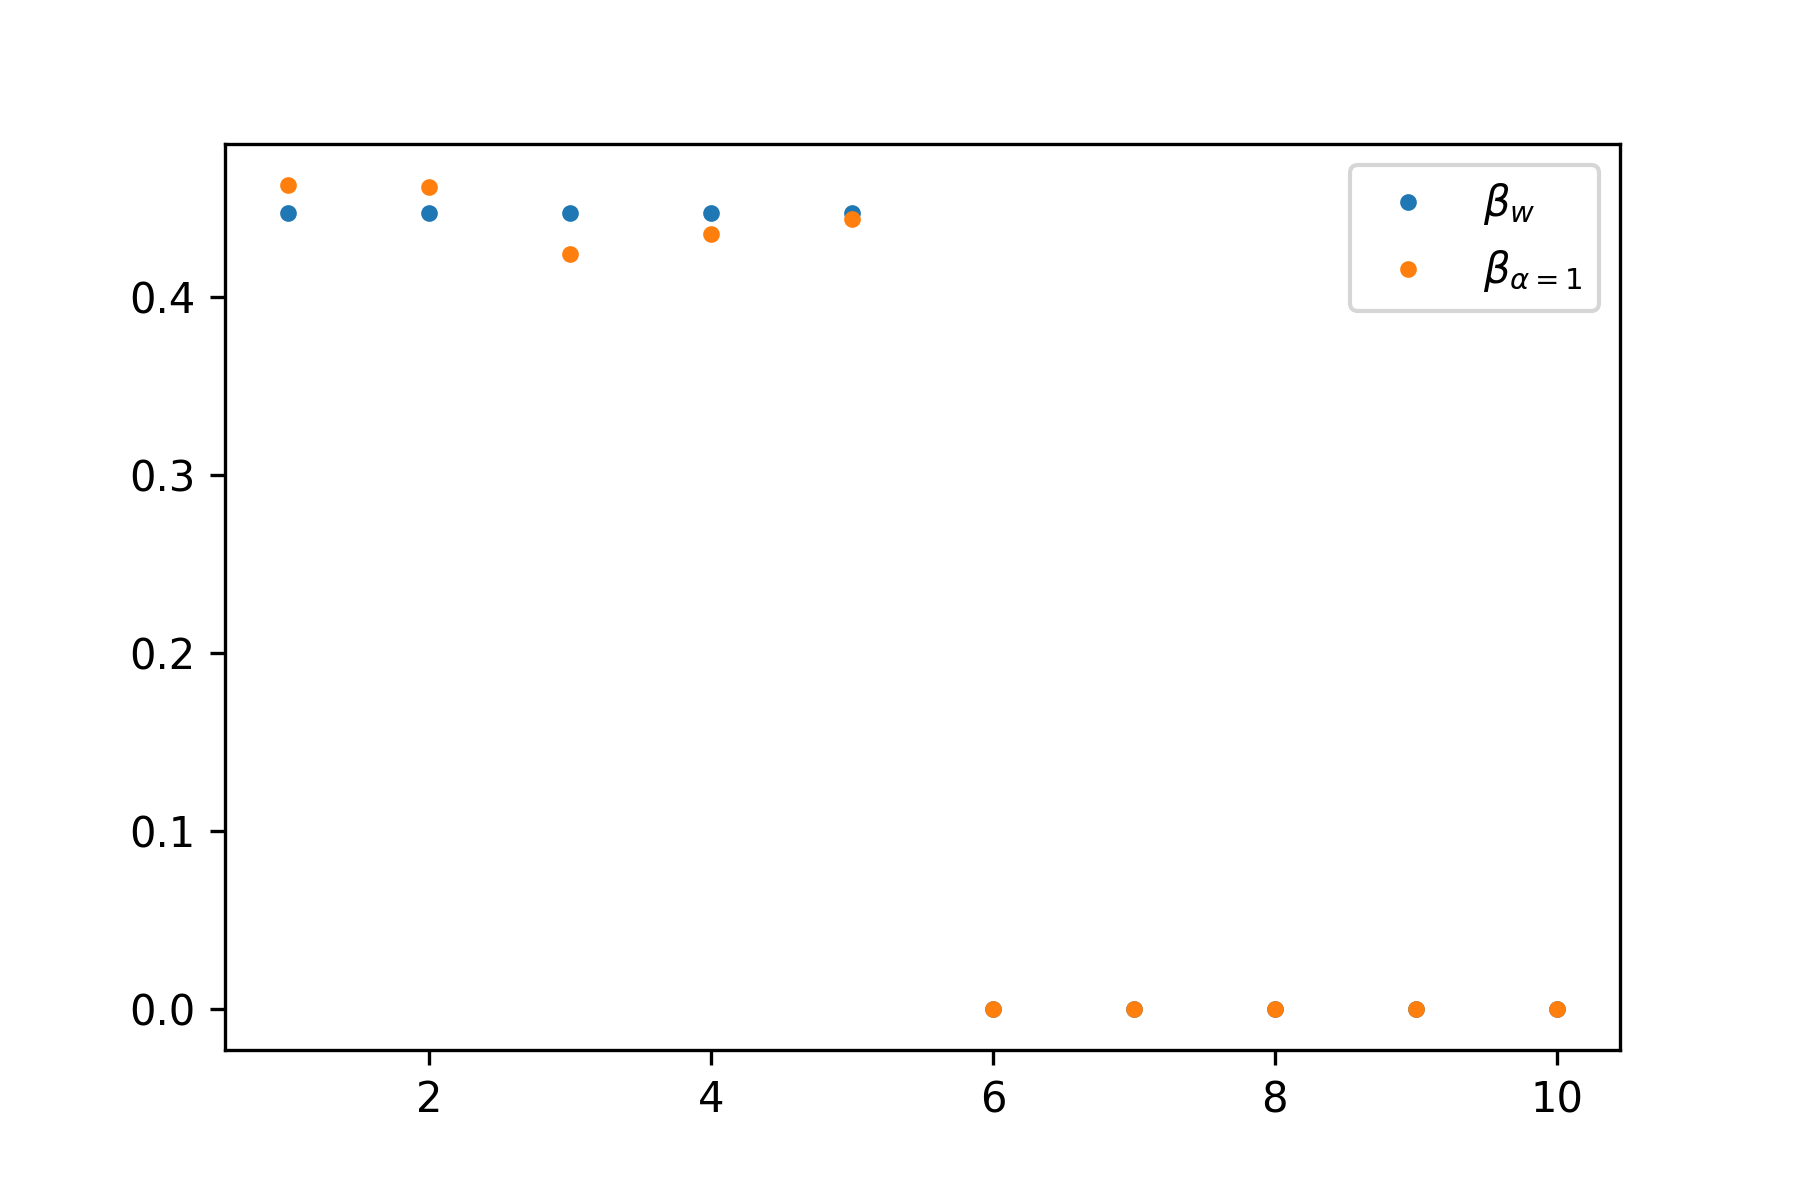
\includegraphics[width=.5\linewidth]{Imgs/Sparse Linear Regression/visualize_solution_vec_0.001.png}\label{}}\hfill
    \subfloat[$\alpha =1$]{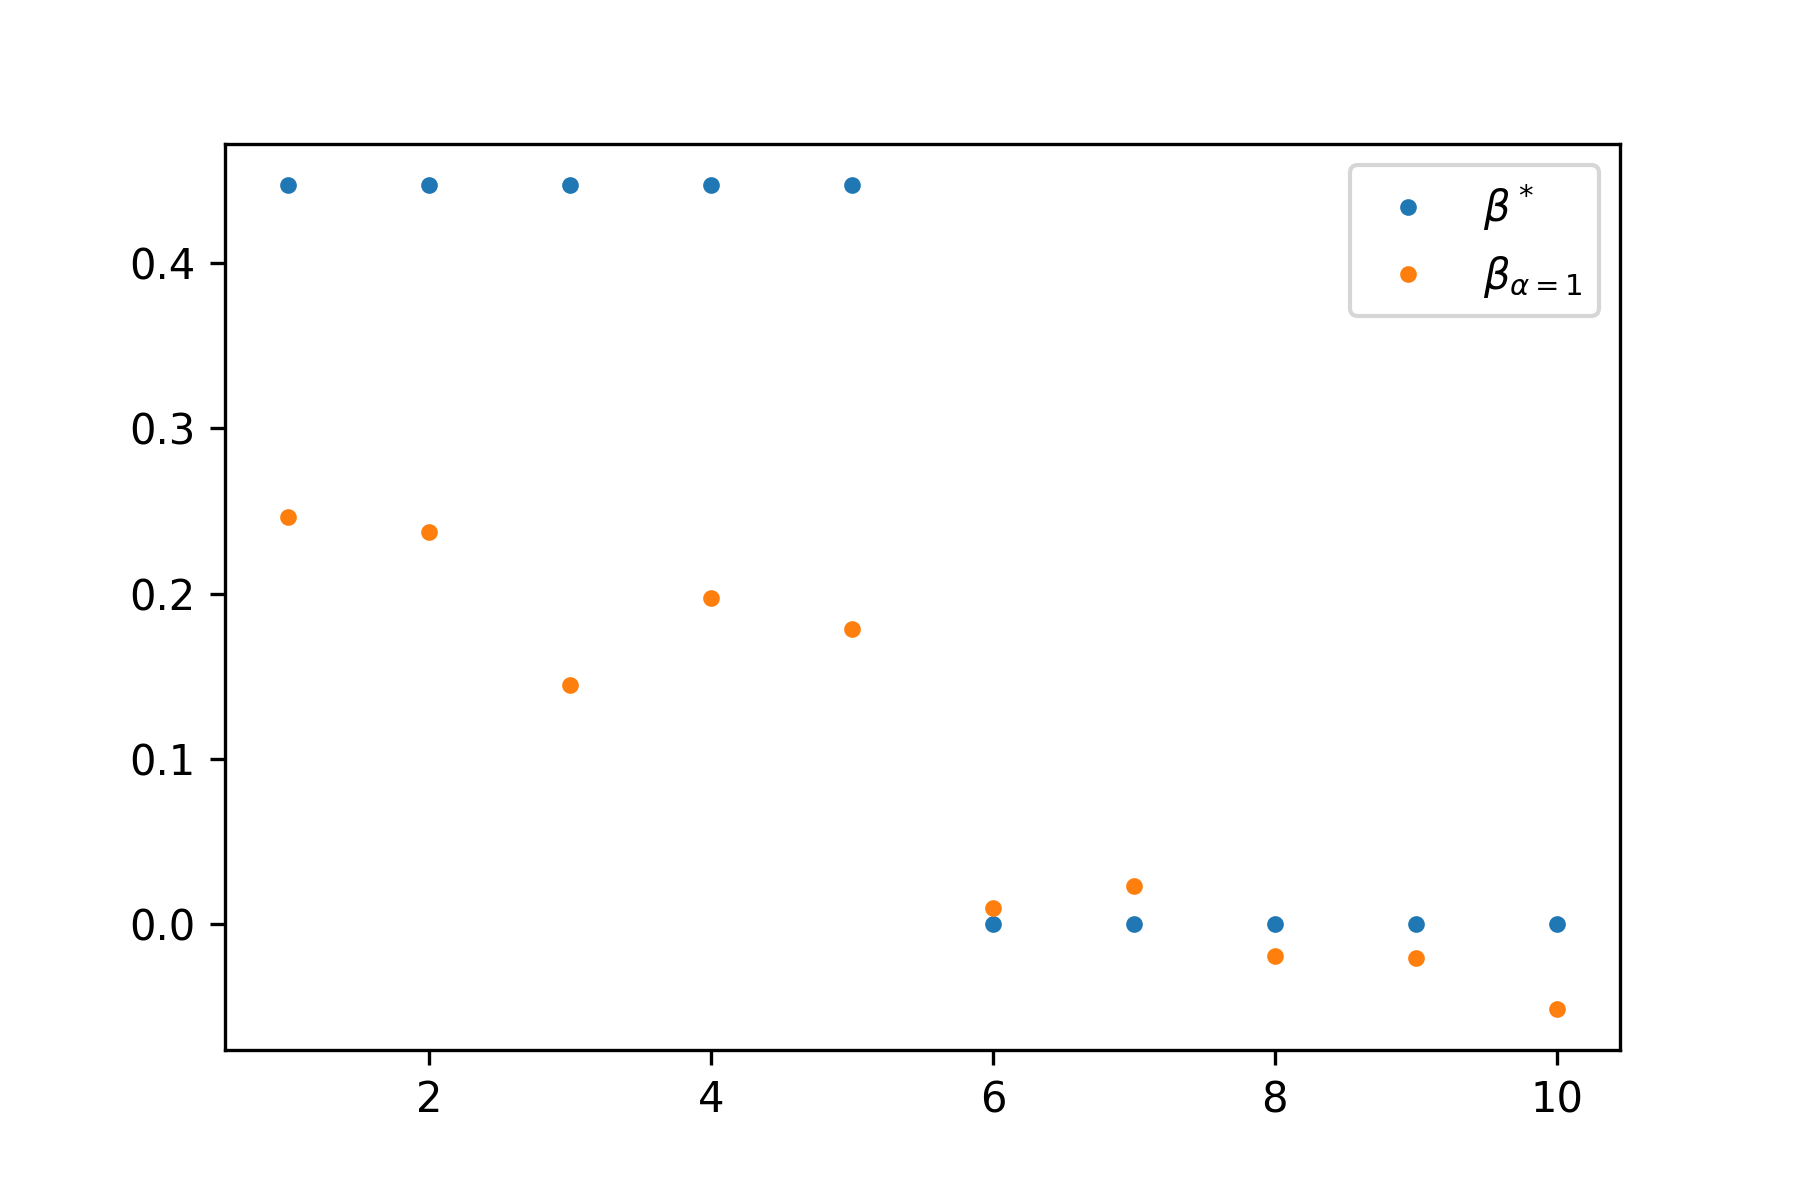
\includegraphics[width=.5\linewidth]{Imgs/Sparse Linear Regression/visualize_solution_vec_1.png}\label{}}
    \caption{The first 10 coordinates of the gradient descent solution vector $\boldsymbol{\beta}_{\boldsymbol{w}_{\alpha}(t_{\text{end}})}$ (orange) and those of the ground truth vector $\boldsymbol{\beta}_{\boldsymbol{w}}$ (blue). Gradient descent is performed using $N=100$ training points.}\label{fig:solutionpts}
\end{figure}

To better visualize how the gradient flow solution changes as a function of the initialization scale, we plot the first 10 coordinates of $\boldsymbol{\beta}_{\boldsymbol{w}_{\alpha}(t_{\text{end}})}$ against those of $\boldsymbol{\beta}_{\boldsymbol{w}}$ for each of $\alpha = 10^{-3}$ and $\alpha = 1$. What first sticks out to us is that the gradient descent solution corresponding to $\alpha = 1$ is not sparse. Although the solution vector certainly exhibits shrinkage of the second five coordinates, they are not close to zero as they are in $\boldsymbol{\beta}_{\boldsymbol{w}}$. For the $\alpha = 10^{-3}$ solution vector, on the other hand, we do observe that the second five coordinates are all nearly zero. Also, the gradient descent solution picks out the first five coordinates as those which are most important for predicting $y_i$, as is the case in the ground truth vector $\boldsymbol{\beta}_{\boldsymbol{w}}$. Not only does it identify these coordinates, but $(\boldsymbol{\beta}_{\boldsymbol{w}_{\alpha}(t_{\text{end}})})_i$ is very close to the $(\boldsymbol{\beta}_{\boldsymbol{w}})_i = 1/\sqrt{5}$ for $1 \leq i \leq 5$. 

It is also worth mentioning that these experimental results agree with those originally reported by Woodworth and colleagues in \cite{woodworth2020kernel}. We carefully chose our input dimension $n$, data distribution $\rho$, and learning rate $\eta$ to match with those used by the authors in Figures 1(c) and 3(c). The problem considered in Figures 1(a) and 1(b) uses $N=100$ training samples, just as we did, but has higher input dimension, $d=10^3$, than that which we considered. Irrespective of this difference in dimension, we observe the same relationship between the initialization scale $\alpha \in \mathbb{R}_{++}$ of the gradient descent path $(\boldsymbol{w}_{\alpha}(t))_{t \geq 0}$ and the population error. Expressly, the authors illustrate that beginning at $\alpha \approx 10^{-1}$ there is a sharp decrease in the population error $\| \boldsymbol{\beta}_{\boldsymbol{w}_{\alpha}(t_{\text{end}})} - \boldsymbol{\beta}_{\boldsymbol{w}} \|_2^2$. And as the initialization scale $\alpha \rightarrow 0$, the population error appears to decrease monotonically towards $0$, albeit at a slower rate. One will notice that the definition of \enquote{population error} adopted by Woodworth and colleagues, the $\ell^2$ difference between $\boldsymbol{\beta}_{\boldsymbol{w}_{\alpha}(t_{\text{end}})}$ and $\boldsymbol{\beta}_{\boldsymbol{w}}$, differs from that we report in Figure \ref{fig:l1populationerror}. 

Similarly, in Figure 1(b) of \cite{woodworth2020kernel}, the authors plot the excess $\ell^1$ norm of the gradient descent solution vector $\boldsymbol{\beta}_{\boldsymbol{w}_{\alpha}(t_{\text{end}})}$. Just as we see from our own experiments in Figure \ref{fig:excessl1error}, starting once again at around $\alpha \approx 10^{-1}$, there is a sharp decrease in the excess $\ell^1$ norm. It then appears to continue decreasing monotonically as $\alpha \rightarrow 0$. As we have mentioned before, because we know that $\boldsymbol{\beta}_{\alpha}^* \rightarrow \boldsymbol{\beta}^{\ell^1}$ as $\alpha \rightarrow \infty$, where $\boldsymbol{\beta}_{\alpha}^* = \lim_{t \to \infty} \boldsymbol{\beta}_{\boldsymbol{w}_{\alpha}(t)}$, then we would expect the excess $\ell^1$ norm of the gradient descent solution to approach $0$ as $\alpha \rightarrow 0$.

In summary, reproducing the work of Woodworth and colleagues, we have suggested a problem in which training near the rich limit is preferable to training near the kernel limit. In particular, we have shown that for the linear regression problem \ref{linreg}, the rich limit corresponds to the minimum $\ell^1$ solution to the system $\boldsymbol{X}\boldsymbol{\beta} = \boldsymbol{y}$, whereas the kernel limit corresponds to the minimum $\ell^2$ solution. Accordingly, we would expect that for problems in which the underlying data distribution $\rho$ is sparse, training our network $f(\boldsymbol{w}, \boldsymbol{x})$ near the rich limit would achieve smaller population risk than had the model been trained near the kernel limit.

\subsubsection{Computational Limitations of Rich Training}


\section{Conclusion}

\begin{figure}[H]
\centering
\subfloat[$\alpha = 10^{-1}$]{\includegraphics[width=.45\linewidth]{Imgs/Sparse Lof}}\hfill
\subfloat[$\alpha = 1$]{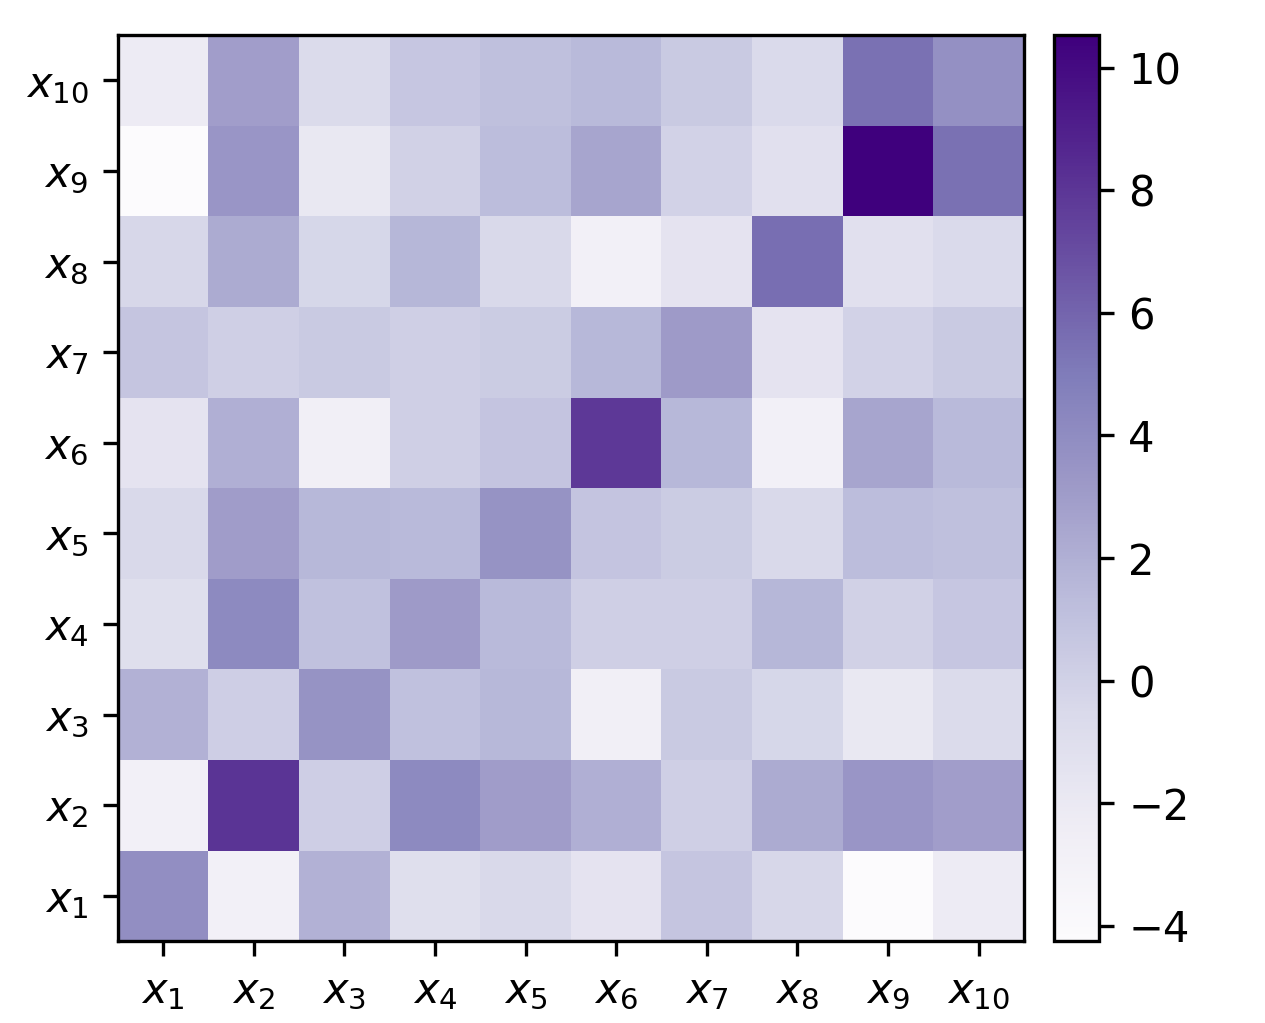
\includegraphics[width=.45\linewidth]{Imgs/NTK/NTK_1/NTK_1_change_total_cropped.png}}\par 
\subfloat[$\alpha = 10^{1}$]{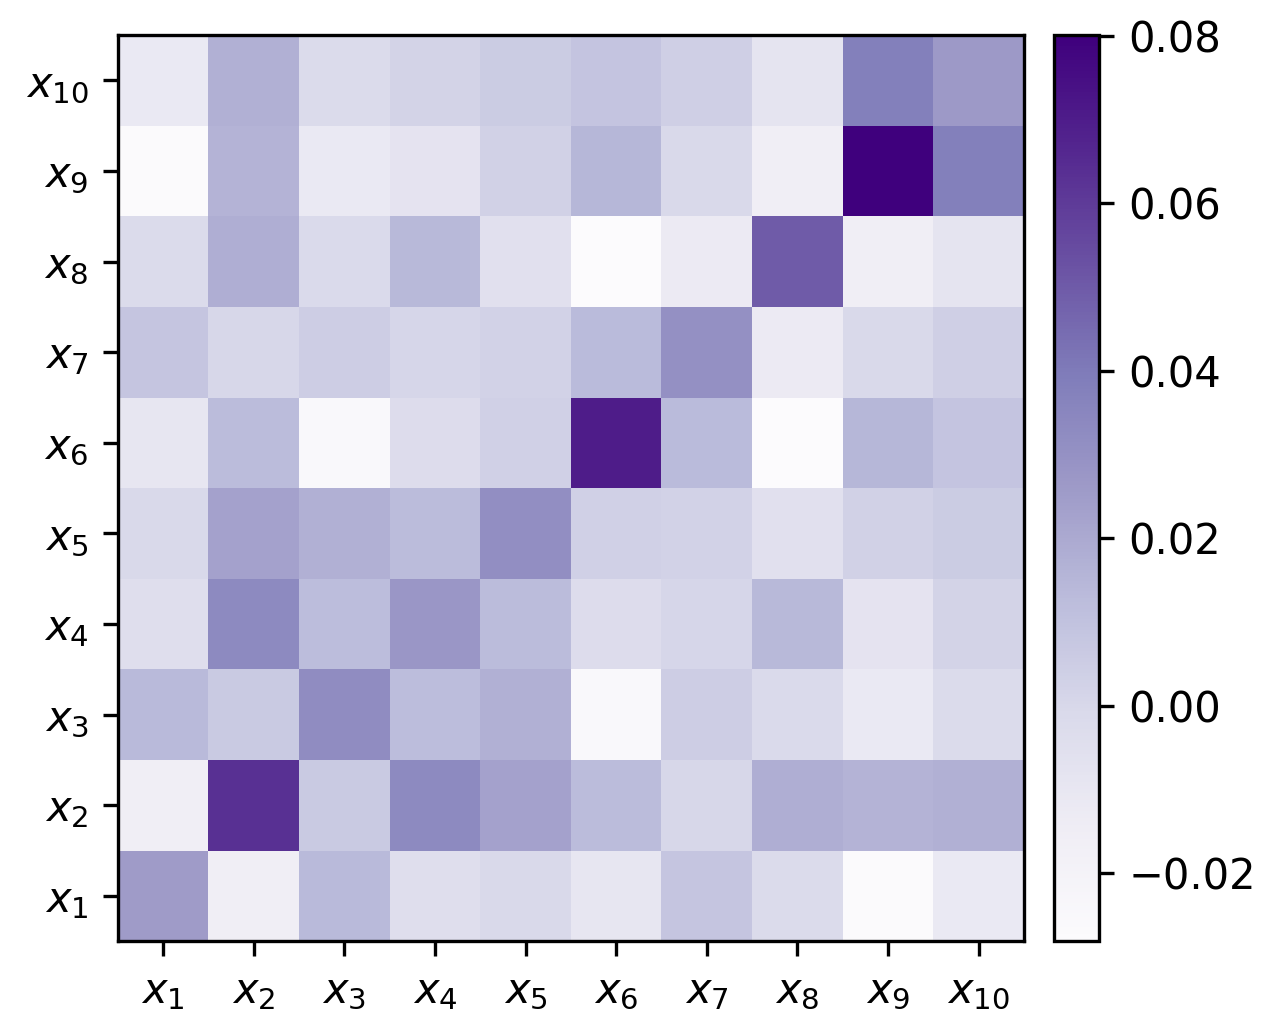
\includegraphics[width=.45\linewidth]{Imgs/NTK/NTK_10/NTK_10_change_total_cropped.png}}
\caption{The change in the neural tangent kernel (NTK) on the grid of $N= 10$ training points $\{ \boldsymbol{x}_i \}_{i=1}^{10}$ throughout training with gradient descent. For each of $\alpha = 10^{-1}, \ 1, \ 10^{1}$, we display the difference between the NTK at initialization $\boldsymbol{w}_{\alpha}(0)$ and at the end of training $\boldsymbol{w}_{\alpha}(t_{\text{end}})$.}\label{img:ntkchange}
\end{figure}

\pagebreak
% References

\bibliographystyle{siam}
\bibliography{References/biblio}

\end{document}